% ============================================================
%  THE MIDNIGHT BREWER -- VOLUME ZERO
%  Setting Everything Up
%
%  Build:  make      (or: latexmk -pdf setup-book.tex)
% ============================================================
\documentclass[11pt,twoside,openright]{book}

% ============================================================
%  The Midnight Brewer -- preamble / design system
%  Compile with: pdflatex (or latexmk -pdf)
% ============================================================

\usepackage[T1]{fontenc}
\usepackage[utf8]{inputenc}

% ---- fonts -------------------------------------------------
\usepackage[mono=false]{libertinus}      % body serif
\usepackage[scaled=0.92]{FiraSans}       % headings sans
\usepackage[scaled=0.86]{sourcecodepro}  % code mono
\usepackage{microtype}

% ---- page geometry -----------------------------------------
\usepackage[
  paperwidth=7.5in, paperheight=9.25in,
  inner=0.95in, outer=0.85in,
  top=0.95in, bottom=1.0in,
  headsep=18pt, footskip=28pt
]{geometry}

\usepackage{graphicx}
\usepackage{amssymb}      % \square for checklists
\usepackage{booktabs}
\usepackage{array}
\usepackage{longtable}
\usepackage{multirow}
\usepackage{enumitem}
\usepackage{xcolor}
\usepackage{tikz}
\usetikzlibrary{positioning,arrows.meta,calc,shapes.geometric,fit,backgrounds,decorations.pathreplacing}
\usepackage[most]{tcolorbox}
\usepackage{listings}
\usepackage{fancyhdr}
\usepackage{titlesec}
\usepackage{makeidx}
\usepackage{emptypage}
\usepackage[bottom]{footmisc}

\usepackage[
  colorlinks=true,
  linkcolor=brewerlink,
  urlcolor=brewerlink,
  citecolor=brewerlink,
  pdftitle={The Midnight Brewer},
  pdfsubject={Building a contactless payment terminal from scratch},
  pdfauthor={Martin},
  bookmarksnumbered=true
]{hyperref}

\makeindex

% ---- palette -----------------------------------------------
\definecolor{brewerink}   {HTML}{16161D}  % near-black body
\definecolor{brewernavy}  {HTML}{1B2A4A}  % headings
\definecolor{brewerlink}  {HTML}{1F5C99}
\definecolor{breweramber} {HTML}{B26B00}  % analogy
\definecolor{brewerred}   {HTML}{A32C2C}  % traps
\definecolor{brewergreen} {HTML}{1F6B4A}  % verification
\definecolor{brewerblue}  {HTML}{27548A}  % concepts
\definecolor{brewergrey}  {HTML}{5A5F6B}
\definecolor{rulegrey}    {HTML}{C9CCD2}
\definecolor{codebg}      {HTML}{F7F7F9}
\definecolor{codeframe}   {HTML}{DDDFE4}
\definecolor{kwcolor}     {HTML}{7A3E9D}
\definecolor{strcolor}    {HTML}{1F6B4A}
\definecolor{comcolor}    {HTML}{6B7280}
\definecolor{todocolor}   {HTML}{B26B00}

\color{brewerink}

% ---- headings ----------------------------------------------
\titleformat{\part}[display]
  {\normalfont\sffamily\bfseries\color{brewernavy}}
  {\Large\MakeUppercase{Part \thepart}}{14pt}{\Huge}
\titleformat{\chapter}[display]
  {\normalfont\sffamily\bfseries\color{brewernavy}}
  {\normalsize\sffamily\mdseries\color{brewergrey}\MakeUppercase{Chapter \thechapter}}
  {8pt}{\LARGE\raggedright}
  [\vspace{4pt}{\color{rulegrey}\rule{\linewidth}{0.6pt}}]
\titleformat{\section}
  {\normalfont\sffamily\bfseries\large\color{brewernavy}}{\thesection}{0.7em}{}
\titleformat{\subsection}
  {\normalfont\sffamily\bfseries\normalsize\color{brewernavy}}{\thesubsection}{0.6em}{}
\titlespacing*{\chapter}{0pt}{6pt}{22pt}
\titlespacing*{\section}{0pt}{18pt}{6pt}
\titlespacing*{\subsection}{0pt}{13pt}{4pt}

% ---- running heads -----------------------------------------
\pagestyle{fancy}
\fancyhf{}
\renewcommand{\headrulewidth}{0.4pt}
\renewcommand{\headrule}{\hbox to\headwidth{\color{rulegrey}\leaders\hrule height \headrulewidth\hfill}}
\fancyhead[LE]{\sffamily\small\color{brewergrey}\leftmark}
\fancyhead[RO]{\sffamily\small\color{brewergrey}\rightmark}
\fancyfoot[C]{\sffamily\small\color{brewergrey}\thepage}
\renewcommand{\chaptermark}[1]{\markboth{\textsc{The Midnight Brewer}}{}}
\renewcommand{\sectionmark}[1]{\markright{#1}}
\fancypagestyle{plain}{\fancyhf{}\renewcommand{\headrulewidth}{0pt}%
  \fancyfoot[C]{\sffamily\small\color{brewergrey}\thepage}}

% ---- code listings -----------------------------------------
\lstdefinestyle{brewerbase}{
  basicstyle=\ttfamily\footnotesize,
  backgroundcolor=\color{codebg},
  frame=single,
  rulecolor=\color{codeframe},
  framesep=6pt,
  xleftmargin=10pt, xrightmargin=0pt,
  breaklines=true,
  breakatwhitespace=false,
  breakindent=14pt,
  postbreak=\mbox{\textcolor{brewergrey}{$\hookrightarrow$}\space},
  columns=fullflexible,
  keepspaces=true,
  showstringspaces=false,
  tabsize=4,
  upquote=true,
  aboveskip=10pt, belowskip=8pt,
  keywordstyle=\color{kwcolor}\bfseries,
  commentstyle=\color{comcolor}\itshape,
  stringstyle=\color{strcolor},
  numberstyle=\tiny\color{brewergrey},
  literate=%
    {á}{{\'a}}1 {é}{{\'e}}1 {í}{{\'i}}1 {ó}{{\'o}}1 {ú}{{\'u}}1
    {€}{{\texteuro}}1 {—}{{---}}1 {–}{{--}}1 {'}{{'}}1
    {“}{{``}}1 {”}{{''}}1 {…}{{\ldots}}1 {×}{{$\times$}}1
    {⚠}{{!}}1 {→}{{$\rightarrow$}}1 {‖}{{$\|$}}1 {≥}{{$\geq$}}1
}

\lstdefinestyle{java}{style=brewerbase,language=Java,
  morekeywords={var,record,sealed,permits,yield},
  moredelim=[il][\color{todocolor}\bfseries]{//!},
}
\lstdefinestyle{dart}{style=brewerbase,language=Java,
  morekeywords={Future,async,await,final,var,late,Uint8List,int,void,class,extends},
}
\lstdefinestyle{bash}{style=brewerbase,language=bash,
  keywordstyle=\color{brewernavy}\bfseries,
}
\lstdefinestyle{xml}{style=brewerbase,language=XML,
  morestring=[b]",
}
\lstdefinestyle{plain}{style=brewerbase,
  keywordstyle=\color{brewerink},
  basicstyle=\ttfamily\scriptsize,
}

\lstset{style=java}

% shorthand environments
\lstnewenvironment{jcode}[1][]{\lstset{style=java,#1}}{}
\lstnewenvironment{dcode}[1][]{\lstset{style=dart,#1}}{}
\lstnewenvironment{shell}[1][]{\lstset{style=bash,#1}}{}
\lstnewenvironment{xcode}[1][]{\lstset{style=xml,#1}}{}
\lstnewenvironment{trace}[1][]{\lstset{style=plain,#1}}{}

% inline code
\newcommand{\code}[1]{\texttt{\small #1}}
\newcommand{\hex}[1]{\texttt{\small #1}}
\newcommand{\reg}[1]{\textsf{\small #1}}

% ---- callout boxes -----------------------------------------
\newtcolorbox{analogybox}[1][]{
  enhanced, breakable,
  colback=breweramber!5, colframe=breweramber,
  borderline west={2.6pt}{0pt}{breweramber},
  frame hidden, arc=0pt, outer arc=0pt,
  boxrule=0pt, left=10pt, right=10pt, top=8pt, bottom=8pt,
  fonttitle=\sffamily\bfseries\small\color{breweramber},
  title={ANALOGY}, attach title to upper={\par\vspace{3pt}},
  #1
}

\newtcolorbox{trapbox}[1][]{
  enhanced, breakable,
  colback=brewerred!4, colframe=brewerred,
  borderline west={2.6pt}{0pt}{brewerred},
  frame hidden, arc=0pt, outer arc=0pt,
  boxrule=0pt, left=10pt, right=10pt, top=8pt, bottom=8pt,
  fonttitle=\sffamily\bfseries\small\color{brewerred},
  title={TRAP}, attach title to upper={\par\vspace{3pt}},
  #1
}

\newtcolorbox{conceptbox}[1][]{
  enhanced, breakable,
  colback=brewerblue!5, colframe=brewerblue,
  borderline west={2.6pt}{0pt}{brewerblue},
  frame hidden, arc=0pt, outer arc=0pt,
  boxrule=0pt, left=10pt, right=10pt, top=8pt, bottom=8pt,
  fonttitle=\sffamily\bfseries\small\color{brewerblue},
  title={CONCEPT}, attach title to upper={\par\vspace{3pt}},
  #1
}

\newtcolorbox{verifybox}[1][]{
  enhanced, breakable,
  colback=brewergreen!5, colframe=brewergreen,
  borderline west={2.6pt}{0pt}{brewergreen},
  frame hidden, arc=0pt, outer arc=0pt,
  boxrule=0pt, left=10pt, right=10pt, top=8pt, bottom=8pt,
  fonttitle=\sffamily\bfseries\small\color{brewergreen},
  title={VERIFICATION GATE}, attach title to upper={\par\vspace{3pt}},
  #1
}

\newtcolorbox{deepbox}[1][]{
  enhanced, breakable,
  colback=black!3, colframe=brewergrey,
  borderline west={2.6pt}{0pt}{brewergrey},
  frame hidden, arc=0pt, outer arc=0pt,
  boxrule=0pt, left=10pt, right=10pt, top=8pt, bottom=8pt,
  fonttitle=\sffamily\bfseries\small\color{brewergrey},
  title={GOING DEEPER}, attach title to upper={\par\vspace{3pt}},
  #1
}

% titled variants
\newtcolorbox{analogy}[1]{enhanced,breakable,colback=breweramber!5,
  borderline west={2.6pt}{0pt}{breweramber},frame hidden,arc=0pt,boxrule=0pt,
  left=10pt,right=10pt,top=8pt,bottom=8pt,
  title={\sffamily\bfseries\small\color{breweramber}ANALOGY\quad#1},
  attach title to upper={\par\vspace{3pt}},colframe=breweramber}
\newtcolorbox{trap}[1]{enhanced,breakable,colback=brewerred!4,
  borderline west={2.6pt}{0pt}{brewerred},frame hidden,arc=0pt,boxrule=0pt,
  left=10pt,right=10pt,top=8pt,bottom=8pt,
  title={\sffamily\bfseries\small\color{brewerred}TRAP\quad#1},
  attach title to upper={\par\vspace{3pt}},colframe=brewerred}
\newtcolorbox{concept}[1]{enhanced,breakable,colback=brewerblue!5,
  borderline west={2.6pt}{0pt}{brewerblue},frame hidden,arc=0pt,boxrule=0pt,
  left=10pt,right=10pt,top=8pt,bottom=8pt,
  title={\sffamily\bfseries\small\color{brewerblue}CONCEPT\quad#1},
  attach title to upper={\par\vspace{3pt}},colframe=brewerblue}
\newtcolorbox{deeper}[1]{enhanced,breakable,colback=black!3,
  borderline west={2.6pt}{0pt}{brewergrey},frame hidden,arc=0pt,boxrule=0pt,
  left=10pt,right=10pt,top=8pt,bottom=8pt,
  title={\sffamily\bfseries\small\color{brewergrey}GOING DEEPER\quad#1},
  attach title to upper={\par\vspace{3pt}},colframe=brewergrey}

% ---- chapter opener block ----------------------------------
% \chapterbrief{goal}{concept}{you end with}
\newcommand{\chapterbrief}[3]{%
  \begin{tcolorbox}[enhanced, colback=brewernavy!4, colframe=brewernavy!25,
    arc=2pt, boxrule=0.5pt, left=12pt, right=12pt, top=10pt, bottom=10pt,
    before skip=2pt, after skip=18pt]
    \setlength{\parskip}{4pt}
    {\sffamily\bfseries\footnotesize\color{brewernavy}GOAL}\quad #1\par
    {\sffamily\bfseries\footnotesize\color{brewernavy}CONCEPT}\quad #2\par
    {\sffamily\bfseries\footnotesize\color{brewernavy}YOU END WITH}\quad #3
  \end{tcolorbox}}

% ---- misc --------------------------------------------------
\setlist[itemize]{leftmargin=1.35em, itemsep=2pt, topsep=4pt}
\setlist[enumerate]{leftmargin=1.6em, itemsep=2pt, topsep=4pt}
\renewcommand{\arraystretch}{1.22}
\setlength{\parskip}{0.45em}
\setlength{\parindent}{0pt}
\setcounter{secnumdepth}{2}
\setcounter{tocdepth}{1}

% table helpers
\newcolumntype{L}[1]{>{\raggedright\arraybackslash}p{#1}}
\newcommand{\thead}[1]{\textsf{\bfseries\small #1}}

% a "symptom / cause" trap table
\newenvironment{traptable}{%
  \par\vspace{4pt}
  \small
  \begin{longtable}{L{0.42\linewidth} L{0.52\linewidth}}
  \toprule \thead{You see} & \thead{Cause / fix} \\ \midrule
  \endhead
}{%
  \bottomrule
  \end{longtable}
  \normalsize
}


% Volume 0 adds one more callout: a "you should now see this" checkpoint.
\newtcolorbox{checkpoint}[1]{enhanced,breakable,colback=brewergreen!5,
  borderline west={2.6pt}{0pt}{brewergreen},frame hidden,arc=0pt,boxrule=0pt,
  left=10pt,right=10pt,top=8pt,bottom=8pt,
  title={\sffamily\bfseries\small\color{brewergreen}CHECKPOINT\quad#1},
  attach title to upper={\par\vspace{3pt}},colframe=brewergreen}

\begin{document}

% ============================================================
\frontmatter
% ============================================================

\begin{titlepage}
\thispagestyle{empty}
\centering
\vspace*{0.7in}

{\sffamily\fontsize{15}{18}\selectfont\color{brewergrey}
 THE\quad MIDNIGHT\quad BREWER\quad$\cdot$\quad VOLUME ZERO\par}

\vspace{0.45in}
{\color{brewernavy}\rule{3.1in}{1.1pt}}\par
\vspace{0.30in}

{\sffamily\bfseries\fontsize{33}{38}\selectfont\color{brewernavy}
 Setting\\[3pt] Everything\\[3pt] Up\par}

\vspace{0.28in}
{\color{brewernavy}\rule{3.1in}{1.1pt}}\par
\vspace{0.34in}

{\fontsize{13}{18}\selectfont\itshape
 From a blank SD card to a Raspberry Pi that\\
 answers over SSH, builds Java, and talks\\ to an NFC reader.\par}

\vspace{0.5in}

% --- laptop -> ssh -> pi vignette ---
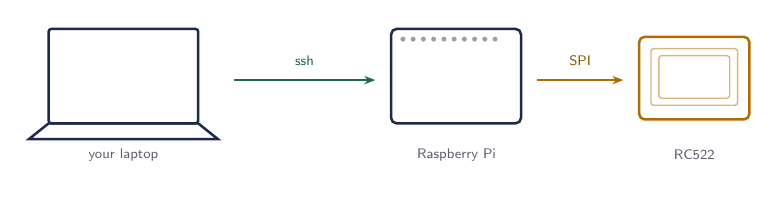
\begin{tikzpicture}[scale=1.0, font=\sffamily\tiny]
  % laptop
  \draw[brewernavy, line width=0.9pt, rounded corners=1pt] (0,0.55) rectangle (1.9,1.75);
  \draw[brewernavy, line width=0.9pt] (-0.25,0.35) -- (2.15,0.35) -- (1.9,0.55) -- (0,0.55) -- cycle;
  \node[color=brewergrey] at (0.95,0.15) {your laptop};
  % ssh arrow
  \draw[-{Stealth[length=4pt]}, brewergreen, line width=0.9pt] (2.35,1.1) -- (4.15,1.1);
  \node[color=brewergreen, above] at (3.25,1.16) {ssh};
  % pi
  \draw[brewernavy, line width=0.9pt, rounded corners=2pt] (4.35,0.55) rectangle (6.0,1.75);
  \foreach \i in {0,...,9}{ \fill[brewergrey!60] (4.5+0.13*\i,1.62) circle (0.9pt); }
  \node[color=brewergrey] at (5.18,0.15) {Raspberry Pi};
  % spi arrow
  \draw[-{Stealth[length=4pt]}, breweramber, line width=0.9pt] (6.2,1.1) -- (7.3,1.1);
  \node[color=breweramber!80!black, above] at (6.75,1.16) {SPI};
  % reader
  \draw[breweramber, line width=0.9pt, rounded corners=2pt] (7.5,0.6) rectangle (8.9,1.65);
  \foreach \i in {0,1}{
    \draw[breweramber!50, line width=0.5pt, rounded corners=1pt]
      (7.65+0.1*\i,0.78+0.09*\i) rectangle (8.75-0.1*\i,1.5-0.09*\i); }
  \node[color=brewergrey] at (8.2,0.15) {RC522};
\end{tikzpicture}

\vfill
{\sffamily\small\color{brewergrey}
 Read this one first\par}
\vspace{6pt}
{\sffamily\footnotesize\color{brewergrey} Revision \today\par}
\end{titlepage}

\cleardoublepage
\thispagestyle{empty}
\vspace*{\fill}
{\small
\textbf{The Midnight Brewer, Volume Zero: Setting Everything Up}\par
\vspace{8pt}
This is the prequel. It assumes you have never used a Raspberry Pi, never
generated an SSH key, and have never run \code{mvn} in your life. It ends with a
Pi you can reach by name, a project that builds, and an NFC reader that
answers.\par
\vspace{10pt}
\textbf{Volume One} --- \emph{Building a Contactless Payment Terminal From
Scratch} --- picks up exactly where this stops, and is where you start writing
code.\par
\vspace{10pt}
\textbf{Every command in this book is meant to be typed.} Where output is shown,
it is what you should actually see. Where it differs, the troubleshooting
appendix is indexed by symptom.\par
}
\vspace*{\fill}

\cleardoublepage
\tableofcontents

\cleardoublepage
\chapter*{Before you start}
\addcontentsline{toc}{chapter}{Before you start}
\markboth{\textsc{Before you start}}{}

Most project tutorials open with ``first, set up your environment'' and then
spend one paragraph on something that will actually take you two evenings and
teach you a dozen things you will use for the rest of your life.

This book is that paragraph, expanded honestly.

\section*{What you will have at the end}

\begin{itemize}
  \item A Raspberry Pi you can reach by typing \code{ssh brewer} --- no
        password, no IP address to remember, from anywhere on your network.
  \item A Java project that compiles on your laptop and runs on the Pi one
        second later.
  \item Your code in git, backed up on GitHub, pushed with one command.
  \item An NFC reader wired up and answering.
\end{itemize}

None of that is specific to this project. Change the word ``NFC'' and you have
the setup for any embedded Linux work you will ever do.

\section*{Who this is for}

Someone who has written some C, can use a text editor, and has never done any of
the following: used SSH, generated a key pair, used git beyond \code{git clone},
run Maven, or set up a headless Linux machine.

If you have done all of those, read Chapter~\ref{ch:need} for the hardware
choices, skim Appendix~\ref{app:cheat}, and go straight to Volume One.

\section*{How this book is different from a wiki page}

\textbf{Everything is explained, not just listed.} You will not be told to run
\code{ssh-keygen -t ed25519} and left to wonder what happened. You will be told
what a key pair \emph{is}, why the private one never moves, and what would
actually go wrong if you skipped it.

That matters because setup steps are exactly the ones you cannot debug by
reading your own code. When SSH refuses you at midnight, understanding
\emph{why} it wants what it wants is the difference between five minutes and an
evening.

\begin{concept}{Checkpoints}
Each chapter ends with a \textbf{checkpoint}: a command to run, and the output
you should see.

\textbf{Do not continue past a failed checkpoint.} Setup problems compound
viciously --- a half-configured SSH key produces errors three chapters later
that look nothing like SSH.
\end{concept}

\section*{Conventions}

Commands are shown with a comment saying \emph{where} to run them, because half
of all setup confusion is running the right command on the wrong machine:

\begin{shell}
# on your laptop
ssh brewer

# on the Pi
ls -l /dev/spidev0.0
\end{shell}

\begin{itemize}
  \item \code{\$USER}, \code{martin}, \code{brewer.local} --- replace with your
        own username and hostname. The book uses \code{martin} and
        \code{brewer} throughout; pick your own in Chapter~\ref{ch:flashing}
        and stay consistent.
  \item \textcolor{brewerred}{Red rules} mark traps that have actually caught
        people. \textcolor{brewerblue}{Blue} explains a concept.
        \textcolor{breweramber}{Amber} is an analogy.
        \textcolor{brewergreen}{Green} is a checkpoint.
\end{itemize}

\section*{If you get stuck}

Appendix~\ref{app:trouble0} is indexed by \textbf{what you see on screen}, not by
topic. Search for your error message there first --- almost every setup failure
in this book has a known cause and a one-line fix.

\vspace{1em}
\begin{flushright}\itshape
Nothing here is hard. Some of it is just unfamiliar.
\end{flushright}


% ============================================================
\mainmatter
% ============================================================

\part{Your Machine}
\chapter{What you need}
\label{ch:need}

\chapterbrief
  {Buy the right things, once.}
  {The decisions that are expensive to change later.}
  {A shopping list and no regrets.}

\section{The shopping list}

\begin{center}\small
\begin{tabular}{@{}L{0.30\linewidth}L{0.42\linewidth}r@{}}
\toprule
\thead{Item} & \thead{Notes} & \thead{Approx.} \\
\midrule
Raspberry Pi Zero 2 W & Any Pi works. See below. & \pounds18 \\
microSD card, 16\,GB+ & Class 10 / A1. A slow card makes everything feel broken. & \pounds8 \\
USB power supply, 5\,V 2.5\,A & \textbf{Not} a phone charger you had lying around. & \pounds8 \\
MFRC522 reader module & The ubiquitous red breakout board. & \pounds3 \\
\textbf{MIFARE DESFire EV2/EV3} & \textbf{Buy two. See the warning.} & \pounds3 ea \\
Female--female jumper wires & Get short ones, 10\,cm. Seriously. & \pounds3 \\
7-inch touchscreen \emph{(optional)} & 1024$\times$600, HDMI $+$ USB touch. Volume One, Chapter 12. & \pounds45 \\
\bottomrule
\end{tabular}
\end{center}

You also need a computer (macOS, Linux or Windows), a home network with Wi-Fi,
and an SD card reader.

\begin{trap}{The card matters more than everything else combined}
It must say \textbf{DESFire EV2} or \textbf{EV3}.

\textbf{Not} MIFARE Classic --- broken crypto, completely different protocol.
\textbf{Not} NTAG or Ultralight --- no crypto at all, no value files.
\textbf{Not} ``13.56\,MHz RFID tag'' from a bag of a hundred on an auction site.

If a listing says ``compatible'' or does not name the chip, it is not one.

\textbf{Buy at least two.} One to develop against, one spare --- because in
Volume One you will run a command that changes a key on the card, and a card
whose key you have changed and forgotten is scrap. Permanently, by design.
\end{trap}

\section{Which Pi?}

Any model with Wi-Fi works. The trade-off:

\begin{center}\small
\begin{tabular}{@{}L{0.24\linewidth}L{0.34\linewidth}L{0.34\linewidth}@{}}
\toprule
\thead{Model} & \thead{Good} & \thead{Annoying} \\
\midrule
Zero 2 W & Cheap, tiny, fits behind a screen & 512\,MB RAM; compiling on it is slow \\
Pi 3 / 4 / 5 & Fast, plenty of RAM & Bigger, more power, more money \\
Zero W (original) & Cheapest & Single core --- genuinely painful. Avoid. \\
\bottomrule
\end{tabular}
\end{center}

This book assumes a \textbf{Zero 2 W}, because it is the one that forces you to
do things properly: with 512\,MB you cannot be careless, and the workflow you
learn in Chapter~\ref{ch:deploy} --- build on the laptop, run on the Pi ---
is the right workflow on any hardware.

Everything works unchanged on a Pi 4; you will just wait less.

\begin{trap}{The power supply is not optional}
A Pi that browns out does not politely stop. It corrupts the SD card, drops the
network, and produces failures that look exactly like software bugs.

If you see random reboots, a rainbow square in the corner, or ``undervoltage
detected'' in \code{dmesg}, replace the supply before debugging anything else. A
phone charger rated ``5\,V 2\,A'' often will not hold 5\,V under load, and the
cable matters as much as the brick.
\end{trap}

\section{Wires: shorter than you think}

Get \textbf{10\,cm female-to-female} jumpers. The 20\,cm ones that come in most
kits are, at the 1\,MHz clock this project uses, genuinely unreliable --- and
their failure mode is intermittent, which is the worst kind.

\begin{analogy}{Shouting across a room}
A short wire is a conversation at arm's length. A long, unshielded, loosely
twisted jumper is shouting across a room with a fan running: most words arrive,
some do not, and you cannot predict which.

Digital signals do not degrade gracefully. A bit that arrives ambiguous is not
``slightly wrong'' --- it is a different number.
\end{analogy}

You will meet this again in Appendix~\ref{app:trouble0}: \emph{version register
reads a different value each run} is almost always wire length, and almost never
code.

\section{What you do not need}

\begin{itemize}
  \item \textbf{A monitor, keyboard or mouse for the Pi.} This book sets it up
        \emph{headless} --- configured before first boot, reached over the
        network. It is faster, and it is how real deployments work.
  \item \textbf{A soldering iron.} The RC522 usually ships with header pins
        already attached. If yours came with loose pins in a bag, you do need to
        solder them, or buy one that is pre-soldered.
  \item \textbf{An Arduino, a level shifter, or a breadboard.} The Pi's GPIO is
        already 3.3\,V, which is what the RC522 wants.
\end{itemize}

\begin{checkpoint}{Before continuing}
You have, physically in front of you: a Pi, an SD card, a power supply, an
RC522, jumper wires, and at least one card that says \textbf{DESFire EV2} or
\textbf{EV3} on the packaging.

If the card is the only thing missing, carry on --- you will not need it until
Chapter~\ref{ch:wiring}.
\end{checkpoint}

\chapter{Your laptop}
\label{ch:laptop}

\chapterbrief
  {Install Java, Maven and git, and prove each one works.}
  {Package managers, and why version numbers matter here.}
  {Three commands that print version numbers.}

Everything in this chapter happens on \textbf{your own computer}, not the Pi.

\section{A package manager first}

Installing software by downloading installers from websites is how you end up
with three Javas and no idea which one runs. Use a package manager: one command
to install, one to update, one to remove.

\subsection*{macOS --- Homebrew}

\begin{shell}
# on your laptop
/bin/bash -c "$(curl -fsSL \
  https://raw.githubusercontent.com/Homebrew/install/HEAD/install.sh)"
\end{shell}

It will ask for your password and print a couple of commands to run afterwards
(adding \code{brew} to your \code{PATH}) --- \textbf{actually run them}, then
close and reopen your terminal.

\subsection*{Linux (Debian/Ubuntu)}

Already installed: \code{apt}.

\subsection*{Windows}

Two options, and this one genuinely matters:

\begin{trap}{Use WSL2, not native Windows}
Install \textbf{WSL2 with Ubuntu} (\code{wsl --install} in an Administrator
PowerShell, then reboot). Do all your work inside that Ubuntu.

Native Windows will fight you on line endings, file permissions, SSH paths and
shell scripts --- four separate categories of confusion that have nothing to do
with what you are trying to learn. Inside WSL2, every command in this book works
exactly as printed.

Keep your project files under the Linux home directory (\code{\textasciitilde/})
and \emph{not} under \code{/mnt/c/}, or filesystem performance will be dreadful.
\end{trap}

\section{Java 21}

\begin{shell}
# macOS
brew install openjdk@21

# Debian / Ubuntu / WSL2
sudo apt update && sudo apt install -y openjdk-21-jdk
\end{shell}

On macOS, Homebrew does not link the JDK where the system expects it. Run the
command it prints, which looks like:

\begin{shell}
sudo ln -sfn /opt/homebrew/opt/openjdk@21/libexec/openjdk.jdk \
             /Library/Java/JavaVirtualMachines/openjdk-21.jdk
\end{shell}

Verify:

\begin{shell}
java -version
\end{shell}

\begin{trace}
openjdk version "21.0.11" 2026-04-21
OpenJDK Runtime Environment (build 21.0.11+10)
OpenJDK 64-Bit Server VM (build 21.0.11+10, mixed mode)
\end{trace}

\begin{concept}{Why 21 specifically}
Java 21 is a \emph{Long Term Support} release, and it has one feature this
project uses constantly: \code{HexFormat}, for parsing and printing hexadecimal
without pulling in a library.

Java 17 would mostly work. Java 11 will not compile the code in Volume One.
Newer than 21 is fine.

If \code{java -version} shows something older, you have two Javas installed and
the wrong one is first in your \code{PATH} --- see
Appendix~\ref{app:trouble0}.
\end{concept}

\section{Maven}

\begin{shell}
# macOS
brew install maven

# Debian / Ubuntu / WSL2
sudo apt install -y maven
\end{shell}

\begin{shell}
mvn -v
\end{shell}

\begin{trace}
Apache Maven 3.9.6
Maven home: /opt/homebrew/Cellar/maven/3.9.6/libexec
Java version: 21.0.11, vendor: Homebrew
\end{trace}

Check that ``Java version'' line --- Maven has its own idea of which Java to use,
and if it says 17 while \code{java -version} says 21, Maven wins and your build
will behave unexpectedly.

\begin{analogy}{What Maven actually does}
Think of \code{pom.xml} as a shopping list plus a recipe.

The shopping list is your dependencies: ``I need Pi4J version 3.0.2''. Maven
fetches them from a central warehouse and caches them in
\code{\textasciitilde/.m2/}, so the second build is offline and instant.

The recipe is the build: compile these sources with this Java version, run these
tests, put the output there. You do not write build steps; you declare what you
want and Maven knows the order.

The first build downloads a lot and feels slow. That is a one-time cost.
\end{analogy}

\section{git}

\begin{shell}
# macOS -- may already be present via Xcode tools
brew install git

# Debian / Ubuntu / WSL2
sudo apt install -y git
\end{shell}

Tell git who you are. This goes into every commit you ever make, so use a real
address:

\begin{shell}
git config --global user.name  "Your Name"
git config --global user.email "you@example.com"

# Name the default branch 'main' -- matches GitHub and this book
git config --global init.defaultBranch main

# Show the config you just set
git config --global --list
\end{shell}

\begin{trap}{Your commit email becomes public}
If you push to a public GitHub repository, every commit shows the email you set
here, forever, in the git history. It is not editable after the fact without
rewriting history.

If that bothers you, GitHub can give you a private no-reply address: find it
under \emph{Settings $\rightarrow$ Emails} and use that instead. Set it now
rather than discovering it in six months.
\end{trap}

\section{One more useful tool}

\code{rsync} copies files efficiently --- only the parts that changed. You will
use it in Chapter~\ref{ch:deploy} to push builds to the Pi.

\begin{shell}
# macOS: already installed
# Debian / Ubuntu / WSL2
sudo apt install -y rsync

rsync --version | head -1
\end{shell}

\begin{checkpoint}{All four tools}
\begin{shell}
java -version     # 21.x
mvn -v            # 3.9.x, reporting Java 21
git --version     # 2.x
rsync --version   # 3.x
\end{shell}

All four print a version. None says ``command not found''. If Maven reports a
different Java version than \code{java -version} does, fix that now ---
Appendix~\ref{app:trouble0} has the two-line solution.
\end{checkpoint}

\chapter{Enough terminal to be dangerous}
\label{ch:terminal}

\chapterbrief
  {The dozen commands this book actually uses.}
  {Paths, permissions, and where you are.}
  {Confidence that you cannot break anything by accident.}

Skip this chapter if \code{cd}, \code{ls}, \code{chmod +x} and \code{sudo} are
already reflexes. Otherwise it is fifteen minutes that will save you hours.

\section{Where am I?}

The shell always has a \emph{current directory}. Almost every confusing error in
setup work comes from being somewhere you did not think you were.

\begin{shell}
pwd                 # print working directory -- where am I?
ls                  # list files here
ls -la              # ... including hidden ones, with details
cd ~/projects       # change directory
cd ..               # up one level
cd -                # back to where I just was
\end{shell}

\begin{concept}{The three special paths}
\begin{description}[leftmargin=0pt, style=nextline]
  \item[\code{\textasciitilde}] your home directory. On the Pi that is
        \code{/home/martin}; on macOS \code{/Users/martin}.
  \item[\code{.}] here, the current directory. \code{./script.sh} means ``the
        script in \emph{this} folder'' --- as opposed to a command found on your
        \code{PATH}.
  \item[\code{..}] one level up.
\end{description}

A path starting with \code{/} is \emph{absolute} --- it means the same thing from
anywhere. Anything else is \emph{relative} to where you currently are, which is
why \code{pwd} is the first thing to check when a command cannot find a file.
\end{concept}

\section{Looking at files}

\begin{shell}
cat file.txt              # dump the whole thing
less file.txt             # page through it (q to quit, / to search)
head -20 file.txt         # first 20 lines
tail -20 file.txt         # last 20 lines
tail -f logfile           # follow it live -- Ctrl-C to stop
grep "error" file.txt     # lines containing "error"
grep -rn "TODO" src/      # search a whole tree, with line numbers
\end{shell}

\code{tail -f} is how you watch a program's log while it runs. You will use it in
Volume One when the kiosk misbehaves.

\section{Editing on the Pi}

You need one editor that works over SSH. \code{nano} is the least painful:

\begin{shell}
nano ~/.bashrc
\end{shell}

Arrow keys move. \textbf{Ctrl-O then Enter} saves. \textbf{Ctrl-X} exits. Those
two shortcuts are all you need, and they are printed at the bottom of the screen
--- where \code{\^{}O} means Ctrl-O.

\begin{trap}{If you find yourself in \texttt{vi}}
Some commands (notably \code{git commit} with no \code{-m}) open a full-screen
editor that ignores everything you type. That is \code{vim}, and it is modal.

To escape: press \textbf{Escape}, then type \textbf{\code{:q!}} and press Enter.
That quits without saving.

To make git use nano instead, permanently:
\begin{shell}
git config --global core.editor nano
\end{shell}
\end{trap}

\section{Permissions, and \texttt{chmod +x}}

Every file carries permissions: who may read it, write it, and \emph{execute} it.

\begin{shell}
ls -l scripts/deploy.sh
\end{shell}

\begin{trace}
-rwxr-xr-x  1 martin  staff  1204 Jul 26 14:02 scripts/deploy.sh
 ^^^
 owner may read, write, execute
\end{trace}

A shell script without the execute bit gives you \code{Permission denied} even
though you can plainly read it. Fix:

\begin{shell}
chmod +x scripts/deploy.sh
\end{shell}

\begin{trap}{Scripts lose the execute bit in transit}
Copy a script through a zip file, a Windows filesystem, or some cloud drives and
the execute bit is silently dropped.

If a script you \emph{know} is fine says \code{Permission denied}, run
\code{chmod +x} on it before suspecting anything else. Git does preserve the
bit, which is one more reason to use git.
\end{trap}

\section{\texttt{sudo}, and when not to use it}

\code{sudo} runs one command as the administrator. Installing packages and
editing system configuration need it. \textbf{Your own project files never do.}

\begin{trap}{Never \texttt{sudo} a build}
If you run \code{sudo mvn compile} even once, the files in \code{target/} end up
owned by root. Your normal user then cannot overwrite them, so the \emph{next}
build fails with a permission error --- and the obvious-looking fix is more
\code{sudo}, which digs the hole deeper.

If it has already happened:
\begin{shell}
sudo chown -R $USER:$USER ~/midnight-brewer
\end{shell}
\end{trap}

\section{Keys that save you}

\begin{center}\small
\begin{tabular}{@{}L{0.22\linewidth}L{0.70\linewidth}@{}}
\toprule
\thead{Key} & \thead{Does} \\
\midrule
\textbf{Tab} & Completes file and command names. Press it constantly. It is also how you check a path exists before pressing Enter. \\
\textbf{Up arrow} & Previous command. Edit and re-run rather than retyping. \\
\textbf{Ctrl-C} & Stop the running program. \\
\textbf{Ctrl-D} & End of input --- also logs you out of SSH. \\
\textbf{Ctrl-R} & Search your command history. Type a few letters of a command you ran last week. \\
\textbf{Ctrl-A / Ctrl-E} & Jump to start / end of the line. \\
\bottomrule
\end{tabular}
\end{center}

\begin{concept}{Tab completion is a correctness tool}
It is not just about typing speed. If Tab does not complete a filename, that
file \emph{does not exist} where you think it does --- and you have found a bug
before running anything.

Beginners type full paths and get ``No such file or directory''. Experienced
people press Tab, see nothing happen, and immediately run \code{ls}.
\end{concept}

\section{Environment variables}

A variable your shell passes to programs it runs. This book uses one:

\begin{shell}
export PI=martin@brewer.local     # set it for this session
echo $PI                          # read it back
\end{shell}

\code{export} only lasts until you close the terminal. To make it permanent, add
the line to your shell's startup file:

\begin{shell}
# which shell am I using?
echo $SHELL

# zsh (macOS default)
echo 'export PI=martin@brewer.local' >> ~/.zshrc

# bash (most Linux, WSL2)
echo 'export PI=martin@brewer.local' >> ~/.bashrc
\end{shell}

Then open a new terminal, or run \code{source \textasciitilde/.zshrc} to apply
it now.

\begin{checkpoint}{Prove the basics}
\begin{shell}
cd ~
pwd                       # prints your home directory
mkdir -p projects/test
cd projects/test
echo "hello" > file.txt
cat file.txt              # prints: hello
ls -l                     # shows file.txt with its permissions
cd ~
rm -rf ~/projects/test    # clean up
\end{shell}

If all of that worked and you understand what each line did, you know enough
terminal for this entire book.
\end{checkpoint}


\part{The Pi}
\chapter{Flashing the Pi, headless}
\label{ch:flashing}

\chapterbrief
  {Write an operating system to the SD card, pre-configured so the Pi joins your Wi-Fi and accepts SSH on first boot.}
  {Headless setup --- no monitor, no keyboard, ever.}
  {A Pi that boots and appears on your network.}

\section{Headless means no screen}

You are never going to plug a monitor into this Pi. Instead you configure it
\emph{before} first boot, and from then on you reach it over the network.

\begin{analogy}{Setting up a phone before you unbox it}
Imagine you could type your Wi-Fi password and set your account name into a
phone \emph{before} it first powered on --- so that the moment it boots it is
already on your network and already yours.

That is what the Raspberry Pi Imager's settings do. The alternative is finding a
spare HDMI cable, a keyboard, and somewhere to put them.
\end{analogy}

\section{Raspberry Pi Imager}

Download it from \code{raspberrypi.com/software} and install it. It runs on
macOS, Windows and Linux.

Insert your SD card, open Imager, and make three choices:

\begin{description}[leftmargin=0pt, style=nextline]
  \item[Device] Your Pi model --- e.g.\ \emph{Raspberry Pi Zero 2 W}.
  \item[Operating System] \textbf{Raspberry Pi OS Lite (64-bit)}, under
        \emph{Raspberry Pi OS (other)}.
  \item[Storage] Your SD card. \textbf{Read this twice.}
\end{description}

\begin{trap}{Imager will happily erase the wrong disk}
It writes to whatever you select and does not undo. Before clicking, confirm the
\emph{size} matches your SD card --- a 32\,GB entry is your card, a 1\,TB entry
is your laptop.

Unplug other external drives while you do this. People have lost backups here.
\end{trap}

\begin{concept}{Why ``Lite'', and why 64-bit}
\textbf{Lite} means no desktop environment. You do not need one --- you will use
SSH --- and on a 512\,MB Zero 2 W a desktop consumes memory your builds need.

\textbf{64-bit} matters because the Java 21 packages are better supported there,
and the JVM performs measurably better.

(Volume One's kiosk chapter does need a graphical desktop. You will install just
the pieces required at that point, rather than carrying a full desktop through
every chapter before it.)
\end{concept}

\section{The settings screen --- the important part}

Before writing, click the \textbf{gear icon} (or answer \emph{``Would you like to
apply OS customisation settings?''} with \textbf{Edit Settings}).

\subsection*{General tab}

\begin{center}\small
\begin{tabular}{@{}L{0.30\linewidth}L{0.62\linewidth}@{}}
\toprule
\thead{Field} & \thead{Set it to} \\
\midrule
Set hostname & \code{brewer} \newline
  {\small This is how you will address the Pi: \code{brewer.local}. Pick
   something short you will not mistype.} \\
Set username and password & Username \code{martin} (or yours), and a real
  password. \newline
  {\small You will only type this password a handful of times before
   Chapter~\ref{ch:sshkeys} replaces it with a key.} \\
Configure wireless LAN & Your Wi-Fi name (SSID) and password, and your
  \textbf{Wireless LAN country} --- required, or Wi-Fi stays off. \\
Set locale settings & Your timezone and keyboard layout. \\
\bottomrule
\end{tabular}
\end{center}

\begin{trap}{The Zero 2 W is 2.4\,GHz only}
It cannot see a 5\,GHz network. If your router presents both bands under
different names, enter the \textbf{2.4\,GHz} one.

If both bands share one name, it usually still works --- but ``the Pi never
appears on the network'' with correct-looking settings is very often this.
\end{trap}

\subsection*{Services tab}

\textbf{Enable SSH}, and choose \textbf{Use password authentication} for now.
You will switch to keys in Chapter~\ref{ch:sshkeys}.

\begin{concept}{What SSH is}
\emph{Secure Shell}: a program that gives you a terminal on another machine over
the network, with everything encrypted in transit.

When you type \code{ssh martin@brewer.local}, you get a shell prompt on the Pi.
Commands you type run \emph{there}. It is the single most important tool in
embedded Linux work, and Chapter~\ref{ch:sshkeys} is entirely about making it
pleasant.
\end{concept}

\section{Write it}

Click \textbf{Save}, then \textbf{Write}, and confirm. It takes a few minutes ---
it writes, then verifies.

When it finishes, macOS may complain that ``the disk you inserted was not
readable''. \textbf{That is normal}: the card now has a Linux filesystem your
laptop cannot read. Eject it and ignore the warning.

\section{First boot}

\begin{enumerate}
  \item Put the SD card in the Pi.
  \item On a Zero 2 W, plug power into the port marked \textbf{PWR IN} --- the
        one nearer the corner. The other is USB data and will not power it.
  \item Wait. \textbf{First boot takes two to three minutes} --- it resizes the
        filesystem and reboots itself once.
\end{enumerate}

The green LED tells you what is happening: irregular flickering is disk
activity, which is good. A steady green light with no flicker for several
minutes usually means it has not booted.

\begin{checkpoint}{The Pi is on the network}
From your laptop:

\begin{shell}
ping brewer.local
\end{shell}

\begin{trace}
PING brewer.local (192.168.1.42): 56 data bytes
64 bytes from 192.168.1.42: icmp_seq=0 ttl=64 time=4.331 ms
\end{trace}

Ctrl-C to stop. Note the IP address --- you may need it in the next chapter.

\textbf{If it does not answer}, wait a full three minutes and try again before
troubleshooting. If it still fails, go to Chapter~\ref{ch:contact}, which is
entirely about finding a Pi that will not answer to its name.
\end{checkpoint}

\chapter{First contact}
\label{ch:contact}

\chapterbrief
  {Find the Pi and log into it.}
  {Hostnames, mDNS, DHCP --- how machines find each other.}
  {A shell prompt that says \code{martin@brewer}.}

\section{Log in}

\begin{shell}
# on your laptop
ssh martin@brewer.local
\end{shell}

The first time, you get this:

\begin{trace}
The authenticity of host 'brewer.local (192.168.1.42)' can't be established.
ED25519 key fingerprint is SHA256:xK3f...9dQ.
Are you sure you want to continue connecting (yes/no/[fingerprint])?
\end{trace}

Type \textbf{\code{yes}} and press Enter. Then your password (it shows nothing as
you type --- that is deliberate, not a broken keyboard).

\begin{trace}
martin@brewer:~ $
\end{trace}

That prompt means you are on the Pi. Everything you type now runs there.

\begin{concept}{What that fingerprint question is}
Every SSH server has its own identity key. The first time you connect, your
computer has no way to know whether this is really your Pi or something
pretending to be it, so it shows you the fingerprint and records your answer in
\code{\textasciitilde/.ssh/known\_hosts}.

From then on it checks silently. If the fingerprint ever \emph{changes}, SSH
refuses to connect and warns loudly --- because that is what an impersonation
attack looks like.

On a home network, the realistic cause of that warning is that you reflashed the
Pi (new key) or your router handed the address to a different device. See
Appendix~\ref{app:trouble0} for the one-line fix --- and note that the fix is to
remove the \emph{specific stale entry}, never to disable checking.
\end{concept}

\section{When \texttt{brewer.local} does not resolve}

\code{.local} names use \textbf{mDNS} --- machines shouting ``I am brewer'' on
the local network, with no central server. It works out of the box on macOS and
most Linux, and on Windows 10+.

When it fails, work down this list.

\subsection{1. Is it a name problem or a network problem?}

Find the Pi's IP from your router's admin page (usually
\code{192.168.1.1} in a browser; look for ``connected devices'' or ``DHCP
leases''). Then:

\begin{shell}
ssh martin@192.168.1.42
\end{shell}

If \textbf{that works}, the Pi is fine and only the name lookup is broken --- fix
it with the \code{\textasciitilde/.ssh/config} entry in
Chapter~\ref{ch:sshkeys}, which lets you type \code{ssh brewer} regardless.

If \textbf{that fails too}, the Pi is not on the network. Continue.

\subsection{2. Scan the network}

\begin{shell}
# macOS / Linux -- find your own address first
ipconfig getifaddr en0        # macOS
hostname -I                   # Linux

# then scan that subnet for open SSH ports
nmap -p 22 --open 192.168.1.0/24
\end{shell}

Install \code{nmap} with \code{brew install nmap} or \code{sudo apt install
nmap}. Any device answering on port 22 is running SSH; if you only have one Pi,
that is it.

\subsection{3. Still nothing}

In order of likelihood:

\begin{center}\small
\begin{tabular}{@{}L{0.42\linewidth}L{0.50\linewidth}@{}}
\toprule
\thead{Cause} & \thead{Check} \\
\midrule
Wi-Fi credentials wrong & Re-flash the card with Imager, retyping the SSID and password carefully. Both are case-sensitive. \\
5\,GHz network selected & A Zero 2 W cannot see 5\,GHz. Use the 2.4\,GHz SSID. \\
Wireless country not set & Imager's \emph{Wireless LAN country} is required; without it the radio stays off. \\
SSH not enabled & Services tab in Imager. Easy to miss. \\
Power & Undervoltage. Try a different supply \emph{and} cable. \\
Card not written & Imager reported an error, or you ejected early. \\
\bottomrule
\end{tabular}
\end{center}

\begin{trap}{Re-flashing is faster than diagnosing}
If the Pi has never appeared, do not spend an hour on it. Re-flash with Imager,
type the Wi-Fi details slowly, and try again. It takes five minutes, and it fixes
the great majority of never-appeared cases.

Diagnosis is worth it once the Pi has worked at least once --- then you know the
hardware is good and something specific changed.
\end{trap}

\section{Look around}

You are logged in. Confirm what you are on:

\begin{shell}
# on the Pi
hostname                              # brewer
whoami                                # martin
cat /proc/device-tree/model; echo     # Raspberry Pi Zero 2 W Rev 1.0
free -h                               # memory: total / used / free
df -h /                               # disk space
uname -m                              # aarch64  <- 64-bit, as intended
ip addr show wlan0 | grep 'inet '     # your IP address
\end{shell}

Two things worth noting now:

\code{free -h} on a Zero 2 W shows about 420\,MB available. That is why
Chapter~\ref{ch:pisetup} adds swap and Chapter~\ref{ch:deploy} builds on your
laptop.

\code{uname -m} must say \code{aarch64}. If it says \code{armv7l} you flashed the
32-bit image --- workable, but re-flash with the 64-bit one now rather than
later.

To leave:

\begin{shell}
exit          # or Ctrl-D
\end{shell}

\section{DHCP, and why the address moves}

Your router hands out addresses on a lease. When the lease expires, or the Pi
reboots, or another device claims it first, the Pi can get a \emph{different}
address.

That is why this book uses \code{brewer.local} rather than a number. If mDNS is
unreliable on your network, the durable fix is a \textbf{static DHCP lease} (also
called an address reservation) in your router: find the Pi in the device list and
tick ``always give this device this address''. Takes a minute, and it is worth
doing before you start filming or demoing anything.

\begin{checkpoint}{You can log in}
\begin{shell}
ssh martin@brewer.local
hostname
exit
\end{shell}

You reached a prompt, it printed \code{brewer}, and you got back out. You typed a
password to do it --- that is what the next chapter fixes.
\end{checkpoint}

\chapter{SSH keys, properly}
\label{ch:sshkeys}

\chapterbrief
  {Replace the password with a key, and make \code{ssh brewer} work from anywhere on your network.}
  {Public-key cryptography, from the user's side.}
  {A one-word login, and no passwords in your workflow.}

This is the chapter that changes how the rest of the project feels. Typing a
password every time you deploy is not merely tedious --- it is the reason people
stop deploying often, and deploying often is the entire point of
Chapter~\ref{ch:deploy}.

\section{What a key pair is}

You generate two mathematically linked files:

\begin{center}
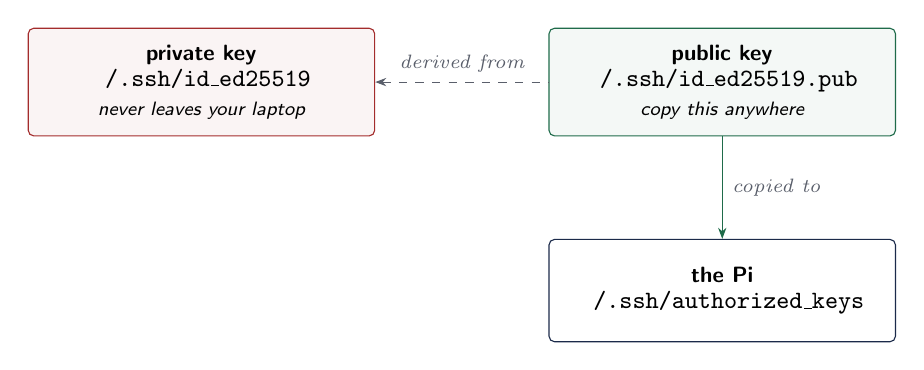
\begin{tikzpicture}[font=\footnotesize\sffamily,
   b/.style={rounded corners=2pt, inner sep=6pt, minimum width=44mm,
             minimum height=13mm, align=center}]
  \node[b, draw=brewerred, fill=brewerred!5] (priv)
       {\textbf{private key}\\ \code{~/.ssh/id\_ed25519}\\[1pt]
        {\scriptsize\itshape never leaves your laptop}};
  \node[b, draw=brewergreen, fill=brewergreen!5, right=22mm of priv] (pub)
       {\textbf{public key}\\ \code{~/.ssh/id\_ed25519.pub}\\[1pt]
        {\scriptsize\itshape copy this anywhere}};
  \draw[{Stealth[length=4pt]}-, brewergrey, dashed] (priv) -- node[above, font=\scriptsize\itshape, color=brewergrey] {derived from} (pub);
  \node[b, draw=brewernavy, below=13mm of pub] (pi)
       {\textbf{the Pi}\\ \code{~/.ssh/authorized\_keys}};
  \draw[-{Stealth[length=4pt]}, brewergreen] (pub) -- node[right, font=\scriptsize\itshape, color=brewergrey] {copied to} (pi);
\end{tikzpicture}
\end{center}

\begin{analogy}{A padlock you hand out freely}
The \textbf{public key} is an open padlock. You can make unlimited copies and
leave them anywhere --- on the Pi, on GitHub, on a colleague's server. A padlock
is not a secret.

The \textbf{private key} is the only key that opens those padlocks. It stays in
one place and is never copied, never emailed, never pasted into a chat.

When you connect, the Pi holds up your padlock and says ``prove you can open
this''. Your laptop proves it \emph{without ever sending the key} --- and that
is the same trick, mathematically, that the DESFire card uses in Volume One,
Chapter 10. You are about to use challenge--response before you implement it.
\end{analogy}

\section{Generate the key}

\begin{shell}
# on your laptop
ssh-keygen -t ed25519 -C "martin@laptop"
\end{shell}

Three questions:

\begin{description}[leftmargin=0pt, style=nextline]
  \item[File to save the key] Press Enter for the default,
        \code{\textasciitilde/.ssh/id\_ed25519}. Only change it if you already
        have a key you want to keep.
  \item[Passphrase] Press Enter twice for none, \emph{or} set one --- see the
        box below.
  \item[Same again] Confirm.
\end{description}

\begin{trace}
Your identification has been saved in /Users/martin/.ssh/id_ed25519
Your public key has been saved in /Users/martin/.ssh/id_ed25519.pub
The key fingerprint is:
SHA256:xK3f...9dQ martin@laptop
\end{trace}

\begin{concept}{\texttt{ed25519}, and passphrases}
\textbf{Why ed25519 and not RSA?} It is a modern elliptic-curve algorithm:
shorter keys, faster, and no key-size decision to get wrong. Use RSA only if you
must talk to something ancient.

\textbf{Should you set a passphrase?} It encrypts the private key on disk, so a
stolen laptop does not hand over your servers. The cost is typing it --- but your
operating system's keychain remembers it after the first use, so in practice you
type it once per reboot.

For a home Pi with nothing valuable on it, no passphrase is a defensible choice.
For the key you will put on GitHub in Chapter~\ref{ch:git}, set one.
\end{concept}

\section{Copy the public key to the Pi}

\begin{shell}
ssh-copy-id martin@brewer.local
\end{shell}

It asks for your Pi password one last time, then:

\begin{trace}
Number of key(s) added: 1

Now try logging into the machine, with:   "ssh 'martin@brewer.local'"
\end{trace}

Test it:

\begin{shell}
ssh martin@brewer.local
\end{shell}

\textbf{No password.} That is the whole point.

\subsection*{If \texttt{ssh-copy-id} is missing (some macOS setups)}

\begin{shell}
brew install ssh-copy-id

# or do it by hand -- this is exactly what the tool does:
cat ~/.ssh/id_ed25519.pub | ssh martin@brewer.local \
  "mkdir -p ~/.ssh && chmod 700 ~/.ssh && \
   cat >> ~/.ssh/authorized_keys && chmod 600 ~/.ssh/authorized_keys"
\end{shell}

\begin{trap}{SSH refuses keys if the permissions are loose}
\code{\textasciitilde/.ssh} must be \code{700} and \code{authorized\_keys} must
be \code{600}. If they are group- or world-writable, the SSH server silently
ignores the key and falls back to asking for a password.

Silently is the operative word: no error, no log line you would notice, just a
password prompt that should not be there. If keys ``do not work'' and you have
checked everything else, check permissions:

\begin{shell}
# on the Pi
chmod 700 ~/.ssh
chmod 600 ~/.ssh/authorized_keys
\end{shell}
\end{trap}

\section{The config file: \texttt{ssh brewer}}

Typing \code{martin@brewer.local} forever is unnecessary. On your laptop, create
\code{\textasciitilde/.ssh/config}:

\begin{shell}
nano ~/.ssh/config
\end{shell}

\begin{trace}
Host brewer
    HostName brewer.local
    User martin
    IdentityFile ~/.ssh/id_ed25519

    # Keep the connection alive through Wi-Fi hiccups instead of
    # dropping you mid-deploy.
    ServerAliveInterval 30
    ServerAliveCountMax 6
\end{trace}

\begin{shell}
chmod 600 ~/.ssh/config
ssh brewer
\end{shell}

That is it. One word.

\begin{concept}{Why this is more than a shortcut}
\code{\textasciitilde/.ssh/config} is read by \emph{everything} that uses SSH ---
\code{scp}, \code{rsync}, \code{git}, and the deploy scripts in
Chapter~\ref{ch:deploy}. Define \code{brewer} once and it works everywhere:

\begin{shell}
scp file.txt brewer:~
rsync -a target/classes/ brewer:midnight-brewer/target/classes/
\end{shell}

It also means that when your Pi's address changes, you edit \emph{one line}
instead of hunting through scripts.

If mDNS is unreliable on your network, put the IP in \code{HostName} instead ---
everything else keeps working unchanged. That indirection is the real value.
\end{concept}

\section{Turn off password logins}

Now that keys work, close the door behind you.

\begin{shell}
# on the Pi
sudo nano /etc/ssh/sshd_config
\end{shell}

Find and set these three (they may exist commented out with a \code{\#} ---
remove it):

\begin{trace}
PasswordAuthentication no
PubkeyAuthentication yes
PermitRootLogin no
\end{trace}

Save (Ctrl-O, Enter), exit (Ctrl-X), then:

\begin{shell}
sudo systemctl restart ssh
\end{shell}

\begin{trap}{Keep your current session open}
\textbf{Do not close your SSH window until you have proved a new one works.}

Open a \emph{second} terminal and run \code{ssh brewer}. If it lets you in, you
are safe. If it does not, you still have the first window to undo the change.

If you close everything and locked yourself out, the recovery is physical: power
off, put the SD card in your laptop, and edit the config on the boot partition
--- or just re-flash. Not fatal, but a genuinely annoying half hour.
\end{trap}

Why bother, on a home network? Because a Pi with password login and a weak
password is exactly what automated scanners look for, and because the habit
matters more than this one machine.

\section{Useful SSH tricks}

\begin{shell}
# run one command without opening a shell
ssh brewer 'uptime'

# copy a file over
scp notes.txt brewer:~

# copy a whole folder back
scp -r brewer:~/logs ./logs

# see what SSH is actually doing, when it misbehaves
ssh -v brewer
\end{shell}

\code{ssh -v} is the diagnostic. It prints every step --- which key it offered,
what the server said --- and it is how you find out that the server ignored your
key because of file permissions.

\begin{checkpoint}{Keys work, passwords are off}
\begin{shell}
# from your laptop, in a NEW terminal
ssh brewer 'hostname && whoami'
\end{shell}

\begin{trace}
brewer
martin
\end{trace}

No password prompt, one word to connect, and the command ran remotely. You are
now set up better than most working developers.
\end{checkpoint}

\chapter{Preparing the Pi}
\label{ch:pisetup}

\chapterbrief
  {Install Java and Maven, enable SPI, join the hardware groups, add swap.}
  {Why a 512\,MB machine needs care.}
  {A Pi that can build and run this project.}

\section{The fast way}

The starter pack ships a script that does everything in this chapter. Read the
chapter anyway --- when something fails later you want to know what was done.

\begin{shell}
# on your laptop, from the template folder
scp scripts/pi-bootstrap.sh brewer:~
ssh brewer 'bash pi-bootstrap.sh'
\end{shell}

Then reboot and skip to the checkpoint:

\begin{shell}
ssh brewer 'sudo reboot'
\end{shell}

The rest of this chapter is the same work, done by hand.

\section{Update first}

\begin{shell}
# on the Pi
sudo apt update
sudo apt full-upgrade -y
\end{shell}

On a Zero 2 W this takes a while on a fresh image. Let it finish.

\begin{concept}{\texttt{update} versus \texttt{upgrade}}
\code{apt update} refreshes the \emph{catalogue} --- what versions exist. It
installs nothing.

\code{apt upgrade} installs newer versions of what you already have.
\code{full-upgrade} additionally allows removing packages when a dependency
requires it, which is what you want on a fresh system.

Running \code{upgrade} without \code{update} first is the most common apt
mistake: it dutifully upgrades to the newest versions it knows about, which may
be months old.
\end{concept}

\section{Java and Maven}

\begin{shell}
sudo apt install -y openjdk-21-jdk maven git rsync
java -version
mvn -v
\end{shell}

\begin{trace}
openjdk version "21.0.11" 2026-04-21
OpenJDK Runtime Environment (build 21.0.11+10-1-deb13u2-Debian)
\end{trace}

Maven on the Pi is used rarely --- Chapter~\ref{ch:deploy} builds on your laptop
--- but it is needed once, to download the dependency jars.

\section{Enable SPI}

SPI is the bus the NFC reader speaks. It is off by default.

\begin{shell}
sudo raspi-config
\end{shell}

Navigate: \textbf{3 Interface Options} $\rightarrow$ \textbf{I4 SPI}
$\rightarrow$ \textbf{Yes} $\rightarrow$ \textbf{Ok} $\rightarrow$
\textbf{Finish}.

Or without the menu:

\begin{shell}
sudo raspi-config nonint do_spi 0      # 0 means ENABLE, confusingly
\end{shell}

\section{Join the hardware groups}

Linux does not let arbitrary programs poke hardware. Access is granted by group
membership.

\begin{shell}
sudo usermod -aG spi,gpio $USER
\end{shell}

\begin{trap}{Group changes need a fresh login}
Your current session still has your \emph{old} groups. Adding yourself to a group
does nothing until you log out and back in --- and over SSH that means
disconnecting, not just opening a new shell.

This produces one of the most confusing errors in the whole setup: you ran the
command, you can see the group in \code{/etc/group}, and the program still says
\code{Permission denied}.

\begin{shell}
exit
ssh brewer
groups          # must now list: spi gpio
\end{shell}
\end{trap}

\section{Swap, on a 512\,MB machine}

A Zero 2 W has 512\,MB of RAM. A JVM plus Maven will exceed that, and when Linux
runs out of memory the kernel starts killing processes --- frequently
\code{sshd}, which locks you out until you power-cycle it.

\begin{shell}
free -h                    # check what you have

sudo dphys-swapfile swapoff
sudo nano /etc/dphys-swapfile
\end{shell}

Change \code{CONF\_SWAPSIZE=100} to \code{CONF\_SWAPSIZE=1024}, then:

\begin{shell}
sudo dphys-swapfile setup
sudo dphys-swapfile swapon
free -h                    # Swap: should now show ~1.0Gi
\end{shell}

\begin{concept}{Swap is a safety net, not speed}
Swap is disk space used as overflow memory. Disk is thousands of times slower
than RAM, so a machine actively swapping is a machine crawling.

That is fine --- the goal is not performance, it is \emph{not dying}. Without
swap, running out of memory kills your SSH session. With swap, it merely gets
slow, and you can still type.

On an SD card, heavy swapping does wear the card. Which is one more argument for
building on your laptop.
\end{concept}

\section{Reboot and verify}

\begin{shell}
sudo reboot
\end{shell}

Wait thirty seconds, reconnect, and check everything:

\begin{shell}
ssh brewer

ls -l /dev/spidev0.0        # the SPI device must exist
groups                      # must include spi and gpio
java -version               # 21.x
free -h                     # swap around 1 GB
uname -m                    # aarch64
\end{shell}

\begin{trace}
crw-rw---- 1 root spi 153, 0 Jul 26 14:02 /dev/spidev0.0
martin adm dialout cdrom sudo audio video plugdev games users input
       render netdev spi gpio lpadmin
\end{trace}

Read that first line: the device is owned by group \code{spi}, and the group has
read/write (\code{rw}). That is exactly why you needed the group membership.

\section{One optional nicety}

Give yourself a clock and a tidy history:

\begin{shell}
# on the Pi
cat >> ~/.bashrc <<'EOF'

# timestamps in history -- surprisingly useful when debugging
export HISTTIMEFORMAT="%F %T  "
export HISTSIZE=5000
export HISTCONTROL=ignoredups

# shortcuts
alias ll='ls -alh'
alias ..='cd ..'
EOF

source ~/.bashrc
\end{shell}

\begin{checkpoint}{The Pi is ready}
\begin{shell}
ssh brewer 'ls -l /dev/spidev0.0 && groups | tr " " "\n" | grep -E "^(spi|gpio)$" && java -version'
\end{shell}

You should see the SPI device, both groups, and Java 21.

If \code{/dev/spidev0.0} does not exist, SPI is not enabled --- rerun
\code{raspi-config} and \emph{reboot}. If the groups are missing, log out and
back in.
\end{checkpoint}


\part{The Workflow}
\chapter{Git and GitHub}
\label{ch:git}

\chapterbrief
  {Put your work under version control and back it up.}
  {Commits as save points; SSH keys, a second time.}
  {\code{git push} working with no password.}

\section{Why bother, on a solo project}

Three reasons, and only the first is the obvious one.

\begin{description}[leftmargin=0pt, style=nextline]
  \item[Backup.] SD cards die. Laptops get spilled on.
  \item[Undo.] Not \code{Ctrl-Z} undo --- \emph{``the reader worked on Tuesday
        and does not now''} undo. Git can show you exactly what changed between
        Tuesday and today.
  \item[A record of your reasoning.] In Volume One each chapter ends with a
        commit. Six months later, \code{git log} is a narrative of what you built
        and in what order --- which is worth more than you expect when you come
        back to it, or film it.
\end{description}

\begin{analogy}{Save points, not autosave}
A word processor autosaves continuously; you cannot go back to ``before I
rewrote that section''.

Git is save points in a game. \emph{You} decide when a moment is worth marking,
and you name it. ``M2: driver reads the version register'' is a save point you
can return to, compare against, or branch from.

The skill is choosing when to save: after something works, before something
risky.
\end{analogy}

\section{Start the repository}

You will do this inside the project folder from Chapter~\ref{ch:project}. If you
have not created it yet, come back after that chapter.

\begin{shell}
# on your laptop, inside the project folder
git init
git status
\end{shell}

\code{git status} is the command you will run most. It answers: what have I
changed, and what is staged?

\section{Your first commit}

\begin{shell}
git add .                 # stage everything not ignored
git status                # confirm what is staged -- always look
git commit -m "chore: project skeleton from the starter pack"
git log --oneline
\end{shell}

\begin{concept}{Why two steps, \texttt{add} then \texttt{commit}}
\code{add} stages changes; \code{commit} records what is staged.

The separation exists so you can commit \emph{part} of your work. You fixed a
bug and also renamed a variable; those are two different stories, and staging
lets you tell them separately.

At first, \code{git add .} then \code{git commit} is fine. Later, \code{git add
-p} steps through each change and asks whether to include it --- and that is when
the two-step design starts earning its keep.
\end{concept}

\subsection*{Commit messages that help later}

A convention worth adopting, because it makes \code{git log} scannable:

\begin{trace}
feat:  a new capability          feat: read the card UID
fix:   a bug fixed               fix: skip the 0x88 cascade tag
chore: housekeeping              chore: add .gitignore
docs:  documentation             docs: explain the FIFO wait loop
test:  tests only                test: RFC 4493 vectors for CMAC
\end{trace}

Write the message as the completion of \emph{``this commit will\ldots''} ---
present tense, imperative. \code{fix: skip the cascade tag}, not \code{fixed the
cascade tag}.

\begin{trap}{What must never be committed}
\code{.gitignore} in the starter pack already excludes \code{target/} and common
secret filenames. Two habits on top of that:

\begin{itemize}
  \item \textbf{Never commit a private key.} \code{id\_ed25519} stays in
        \code{\textasciitilde/.ssh/}, never in a project.
  \item \textbf{Never commit a password.} Not in a config file, not in a
        comment, not ``temporarily''.
\end{itemize}

Git history is permanent. Deleting a secret in a later commit does \emph{not}
remove it --- it is still there in the history, and if you pushed it publicly,
assume it is compromised and rotate it.
\end{trap}

\section{GitHub}

Create an account at \code{github.com} if you do not have one, then a new
repository: \textbf{New} $\rightarrow$ name it \code{midnight-brewer}
$\rightarrow$ \textbf{Private} $\rightarrow$ and \textbf{do not} tick any of
``add a README / .gitignore / licence'' (you already have files; those options
create a conflicting first commit).

\subsection{An SSH key for GitHub}

You can push over HTTPS with a token, but SSH is less friction and you already
know how it works.

\begin{shell}
# on your laptop -- reuse the key you already made
cat ~/.ssh/id_ed25519.pub
\end{shell}

Copy the whole line (it starts \code{ssh-ed25519} and ends with your comment).
In GitHub: \textbf{Settings} $\rightarrow$ \textbf{SSH and GPG keys}
$\rightarrow$ \textbf{New SSH key}, paste, save.

Test:

\begin{shell}
ssh -T git@github.com
\end{shell}

\begin{trace}
Hi evilcomputer12! You've successfully authenticated,
but GitHub does not provide shell access.
\end{trace}

That message is success --- GitHub is not supposed to give you a shell.

\begin{concept}{The same padlock, a second lock}
This is the identical key pair from Chapter~\ref{ch:sshkeys}. You handed a copy
of the public half to your Pi; now you have handed another copy to GitHub.

One private key, many places that recognise it. That is the whole model, and it
is why the private key never moving matters: it is the single thing whose
compromise would unlock everything at once.
\end{concept}

\section{Push}

\begin{shell}
git remote add origin git@github.com:YOURNAME/midnight-brewer.git
git branch -M main
git push -u origin main
\end{shell}

\begin{trace}
Enumerating objects: 14, done.
Writing objects: 100% (14/14), 3.21 KiB | 3.21 MiB/s, done.
To github.com:YOURNAME/midnight-brewer.git
 * [new branch]      main -> main
branch 'main' set up to track 'origin/main'.
\end{trace}

Refresh the GitHub page --- your files are there.

The \code{-u} sets \code{origin/main} as the default, so from now on it is just:

\begin{shell}
git push
\end{shell}

\section{The loop you will actually use}

\begin{shell}
git status                    # what changed?
git diff                      # show me the actual changes
git add -A                    # stage everything
git commit -m "feat: ..."     # save point
git push                      # back it up
\end{shell}

And two that save you:

\begin{shell}
git log --oneline -10         # last ten save points
git diff HEAD~1               # what changed in the last commit
git checkout -- file.java     # throw away my changes to this file
\end{shell}

\begin{trap}{\texttt{git checkout -{}-} is destructive}
That last command discards your uncommitted changes to that file,
\emph{permanently}. There is no undo, because the changes were never recorded.

That is precisely why you commit often: committed work can always be recovered;
uncommitted work is one careless command from gone.
\end{trap}

\begin{checkpoint}{Your code is backed up}
\begin{shell}
git log --oneline
git push
\end{shell}

At least one commit exists, \code{push} reports \emph{Everything up-to-date},
and you can see your files on github.com.
\end{checkpoint}

\chapter{The project skeleton}
\label{ch:project}

\chapterbrief
  {Copy the template, build it, run its tests --- all on your laptop.}
  {What Maven's folder layout means, and why it is not negotiable.}
  {\code{Tests run: 3, Failures: 0}.}

\section{Copy the template}

\begin{shell}
# on your laptop
cp -r starter-pack/template ~/midnight-brewer
cd ~/midnight-brewer
ls -la
\end{shell}

\section{Build it before you change anything}

\begin{shell}
mvn test
\end{shell}

The first run downloads dependencies and takes a minute or two. Afterwards it is
seconds.

\begin{trace}
[INFO] Tests run: 3, Failures: 0, Errors: 0, Skipped: 0
[INFO] BUILD SUCCESS
\end{trace}

\begin{trap}{Read the number, not the word}
\code{BUILD SUCCESS} with \emph{Tests run: 0} is also a success, and it means
your tests are not being found at all.

This is the single most common silent failure in Java projects: a misplaced test
folder, a class not ending in \code{Test}, an old Surefire version that cannot
see JUnit 5. Everything looks green and nothing is verified.

\textbf{Always check the count.} Here it must say 3.
\end{trap}

\section{What is in the folder}

\begin{center}
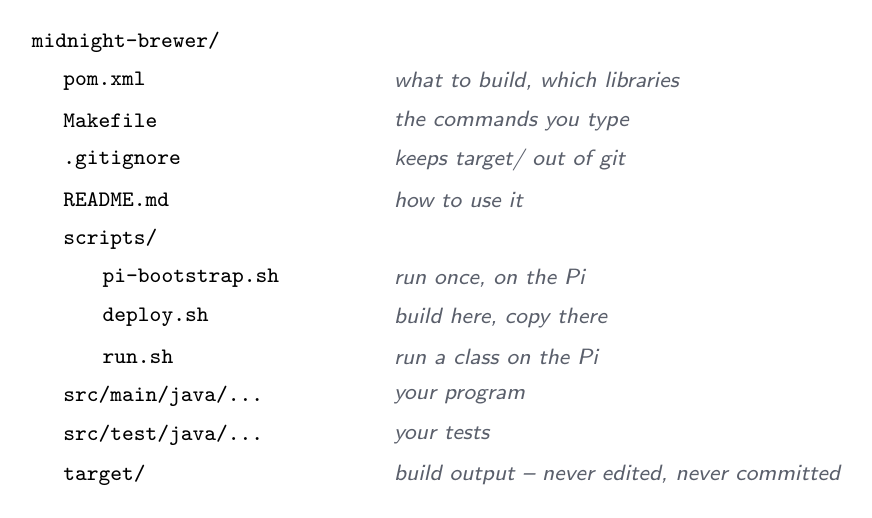
\begin{tikzpicture}[font=\footnotesize\ttfamily, node distance=0mm,
  f/.style={anchor=west, inner sep=1.5pt},
  c/.style={anchor=west, inner sep=1.5pt, font=\footnotesize\sffamily\itshape,
            color=brewergrey}]
  \def\y{0}
  \node[f] at (0,0.0)   {midnight-brewer/};
  \node[f] at (0.4,-0.5) {pom.xml};
    \node[c] at (4.6,-0.5) {what to build, which libraries};
  \node[f] at (0.4,-1.0) {Makefile};
    \node[c] at (4.6,-1.0) {the commands you type};
  \node[f] at (0.4,-1.5) {.gitignore};
    \node[c] at (4.6,-1.5) {keeps target/ out of git};
  \node[f] at (0.4,-2.0) {README.md};
    \node[c] at (4.6,-2.0) {how to use it};
  \node[f] at (0.4,-2.5) {scripts/};
  \node[f] at (0.9,-3.0) {pi-bootstrap.sh};
    \node[c] at (4.6,-3.0) {run once, on the Pi};
  \node[f] at (0.9,-3.5) {deploy.sh};
    \node[c] at (4.6,-3.5) {build here, copy there};
  \node[f] at (0.9,-4.0) {run.sh};
    \node[c] at (4.6,-4.0) {run a class on the Pi};
  \node[f] at (0.4,-4.5) {src/main/java/...};
    \node[c] at (4.6,-4.5) {your program};
  \node[f] at (0.4,-5.0) {src/test/java/...};
    \node[c] at (4.6,-5.0) {your tests};
  \node[f] at (0.4,-5.5) {target/};
    \node[c] at (4.6,-5.5) {build output -- never edited, never committed};
\end{tikzpicture}
\end{center}

\begin{concept}{Why \texttt{src/main/java} and not something shorter}
Maven follows \emph{convention over configuration}: it knows where sources live,
so you never write it down.

Put a file in the wrong place and it is silently not compiled --- no error, it
simply does not exist as far as the build is concerned. That is the trade: total
consistency across every Maven project in the world, at the cost of paths being
fixed.

The package \code{com.midnightbrewer.diag} must map to the folder
\code{src/main/java/com/midnightbrewer/diag/}. Not similar --- identical.
\end{concept}

\section{Run the toolchain check}

\begin{shell}
mvn -q compile
java -cp target/classes com.midnightbrewer.ToolchainCheck
\end{shell}

\begin{trace}
=== toolchain check ===
java.version    = 21.0.11
os.name         = Mac OS X
os.arch         = aarch64
major version   = 21
sanity          = 0x92 (146)

  -> toolchain OK. Nothing above needed hardware.
\end{trace}

\begin{concept}{What \texttt{-cp} means}
\code{-cp} is the \emph{classpath}: where Java looks for compiled classes.

\code{target/classes} is where Maven put your compiled code. Later you will use
\code{-cp "target/classes:target/dependency/*"} to include the library jars as
well --- the colon separates entries, and the \code{*} means ``every jar in that
folder''.

Most ``\code{ClassNotFoundException}'' and ``\code{NoClassDefFoundError}''
problems are a classpath missing an entry, not a missing file.
\end{concept}

\section{Read the test}

Open \code{src/test/java/com/midnightbrewer/ToolchainCheckTest.java}. One test
is worth understanding now, because it encodes the mistake you are most likely
to make in Volume One:

\begin{jcode}
@Test
void signedByteMaskingWorks() {
    byte b = (byte) 0x92;

    assertEquals(-110, b, "a signed byte holding 0x92 reads as -110");
    assertEquals(146, b & 0xFF, "masked with 0xFF it reads as 146");
}
\end{jcode}

Java's \code{byte} is signed and there is no \code{unsigned} keyword. \hex{0x92}
has its top bit set, so read as a number it is $-110$. The idiom \code{\& 0xFF}
promotes to \code{int} and strips the sign extension.

You will forget this at least once. Everyone does.

\section{The Makefile}

\begin{shell}
make            # lists every target
\end{shell}

\begin{trace}
Midnight Brewer -- available targets:

  build        compile locally
  test         run the tests locally
  deploy       build + copy classes to the Pi
  run          run MAIN on the Pi
  probe        run the RC522 wiring probe on the Pi
  pi-setup     copy + run the one-time Pi bootstrap script
  ssh          open a shell on the Pi
\end{trace}

\begin{concept}{Why a Makefile and not just typing the commands}
Because you will type these hundreds of times, and because six months from now
\code{make deploy} still works when you have forgotten the rsync flags.

A Makefile is executable documentation. The commands are recorded in the
repository, they are the same for everyone, and \code{make} with no arguments
tells you what is available --- which is more than most projects manage.
\end{concept}

\section{Point it at your Pi}

\begin{shell}
export PI=martin@brewer
\end{shell}

Add that to \code{\textasciitilde/.zshrc} or \code{\textasciitilde/.bashrc} so it
survives a new terminal. It uses the \code{brewer} alias from your
\code{\textasciitilde/.ssh/config}.

\section{Commit it}

Now do Chapter~\ref{ch:git} if you have not:

\begin{shell}
git init
git add .
git commit -m "chore: project skeleton from the starter pack"
\end{shell}

\begin{checkpoint}{The project builds}
\begin{shell}
cd ~/midnight-brewer
mvn test
make
\end{shell}

\code{Tests run: 3, Failures: 0}, and \code{make} lists its targets.

No hardware has been involved yet. That is the point: when something breaks in
Volume One, you already know the toolchain is not the problem.
\end{checkpoint}

\chapter{The deploy loop}
\label{ch:deploy}

\chapterbrief
  {Build on your laptop, run on the Pi, in about five seconds.}
  {Why the feedback loop's length decides how you work.}
  {\code{make deploy \&\& make run} as one reflex.}

\section{The loop is the thing}

How long it takes to see the effect of a change determines how you behave.

\begin{center}\small
\begin{tabular}{@{}L{0.16\linewidth}L{0.76\linewidth}@{}}
\toprule
\thead{Loop} & \thead{How you end up working} \\
\midrule
5 s   & Try it. Wrong? Change one thing, try again. You experiment. \\
40 s  & You batch up three changes to avoid the wait --- and when it fails you no longer know which one did it. \\
3 min & You stop running it. You read the code and \emph{reason}, which is far more error-prone than looking. \\
\bottomrule
\end{tabular}
\end{center}

The middle row is the dangerous one, because it feels productive.

\begin{analogy}{Tasting while you cook}
A cook tastes constantly --- a pinch of salt, taste, another pinch. Small
corrections, immediate feedback.

Now imagine each taste took three minutes. You would salt once, hopefully, and
find out at the table. That is what a slow build does to programming: it turns
tasting into guessing.
\end{analogy}

\section{Why not just build on the Pi?}

You could. \code{git push} from the laptop, \code{git pull} on the Pi, \code{mvn
compile}. It works, and on a Zero 2 W it takes roughly forty seconds.

The trick is that \textbf{Java bytecode is architecture-independent}. A
\code{.class} file compiled on your laptop --- x86 or Apple Silicon, does not
matter --- runs unchanged on the Pi's ARM chip. The JVM is the portability layer.

So: compile on the fast machine, copy the output to the slow one.

\begin{center}
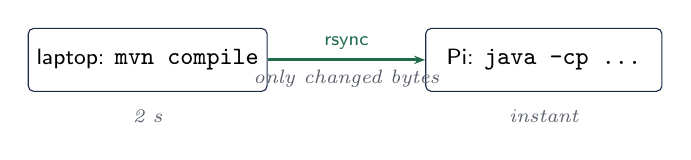
\begin{tikzpicture}[font=\footnotesize\sffamily,
  b/.style={draw=brewernavy, rounded corners=2pt, minimum width=30mm,
            minimum height=8mm, inner sep=3pt}]
  \node[b] (l) {laptop: \code{mvn compile}};
  \node[b, right=20mm of l] (r) {Pi: \code{java -cp ...}};
  \draw[-{Stealth[length=4pt]}, brewergreen, line width=1pt] (l) --
     node[above, font=\scriptsize\sffamily, color=brewergreen] {rsync}
     node[below, font=\scriptsize\itshape, color=brewergrey] {only changed bytes} (r);
  \node[font=\scriptsize\itshape, color=brewergrey, below=1mm of l] {2 s};
  \node[font=\scriptsize\itshape, color=brewergrey, below=1mm of r] {instant};
\end{tikzpicture}
\end{center}

\section{One-time: the dependency jars}

Your code needs Pi4J and SLF4J at runtime. Those jars change only when
\code{pom.xml} changes, so copy them once:

\begin{shell}
# on your laptop, in the project
make deploy-full
\end{shell}

That builds, resolves the dependency jars into \code{target/dependency/}, and
copies both to the Pi.

\section{Every time after that}

\begin{shell}
make deploy
make run
\end{shell}

\begin{trace}
==> building locally
==> copying classes to martin@brewer:~/midnight-brewer
==> done
=== toolchain check ===
java.version    = 21.0.11
os.arch         = aarch64            <- note: you are on the Pi now
major version   = 21
  -> toolchain OK.
\end{trace}

That \code{os.arch = aarch64} is the proof: you compiled on your laptop and the
result ran on ARM.

To run something else:

\begin{shell}
make run MAIN=com.midnightbrewer.diag.SpiProbe
# or equivalently
./scripts/run.sh com.midnightbrewer.diag.SpiProbe
\end{shell}

\section{What the scripts actually do}

Worth reading once, so they are not magic.

\subsection*{\texttt{deploy.sh}}

\begin{shell}
mvn -q -DskipTests compile
rsync -a --delete target/classes/ "$PI:midnight-brewer/target/classes/"
\end{shell}

\begin{description}[leftmargin=0pt, style=nextline]
  \item[\code{-DskipTests}] tests already ran on your laptop; running them again
        on the Pi would be slow and pointless.
  \item[\code{rsync -a}] archive mode: recursive, preserves timestamps and
        permissions.
  \item[\code{-{}-delete}] remove files on the Pi that no longer exist locally.
        Without it, a class you renamed lingers over there --- and stale classes
        produce genuinely baffling behaviour.
  \item[the trailing slashes] \code{target/classes/} means \emph{the contents
        of}. Without the slash rsync would create
        \code{classes/classes/}. This bites everyone once.
\end{description}

\subsection*{\texttt{run.sh}}

\begin{shell}
ssh -t "$PI" "cd ~/midnight-brewer && java -cp 'target/classes:target/dependency/*' $MAIN"
\end{shell}

\code{-t} forces a terminal, so \textbf{Ctrl-C reaches the program on the Pi}
instead of only killing your local ssh client and leaving the program running
over there. Without it you accumulate orphaned processes holding the SPI device,
and the next run fails with a resource-busy error you will not understand.

\begin{trap}{Stale classes}
If you change a file and behaviour does not change, suspect stale output before
suspecting anything else.

\begin{shell}
mvn clean compile && make deploy-full
\end{shell}

The symptom is unmistakable once you know it: the code in front of you
\emph{cannot} produce the output you are seeing.
\end{trap}

\section{The rhythm}

\begin{shell}
# edit code in your editor
mvn test                 # fast, local, no hardware
make deploy && make run  # on the real thing
\end{shell}

Most of your loop is the middle line. The bottom line is for when you need
actual hardware --- and by Volume One, Chapter 1, you will have arranged for that
to be as rarely as possible.

\begin{checkpoint}{The loop works}
\begin{shell}
make deploy-full
make run
\end{shell}

You see the toolchain check, printed by the Pi, reporting \code{aarch64}.

Now change one line in \code{ToolchainCheck.java} --- add a
\code{System.out.println("hello from the loop");} --- and run:

\begin{shell}
make deploy && make run
\end{shell}

Your new line appears. Time it: it should be around five seconds. That number is
what the rest of the project will feel like.
\end{checkpoint}

\chapter{An editor that helps}
\label{ch:editor}

\chapterbrief
  {Set up an editor that understands Java, so mistakes surface as you type.}
  {What a language server does for you.}
  {Autocomplete, red squiggles, and jump-to-definition.}

\section{Why this matters more in Java than in C}

Java is verbose, and a good editor absorbs most of that verbosity: it writes the
imports, completes the method names, and underlines the type error before you
compile.

Without one, you will spend a real fraction of Volume One fixing errors an editor
would have shown you as you typed. With one, Java stops feeling wordy.

\section{VS Code, the pragmatic default}

Free, works everywhere, and its remote-SSH support is genuinely excellent.

\begin{enumerate}
  \item Install from \code{code.visualstudio.com}.
  \item Open the Extensions panel (the four-squares icon) and install
        \textbf{Extension Pack for Java} by Microsoft. That single pack pulls in
        the language server, debugger, Maven and test support.
  \item Open your project: \textbf{File $\rightarrow$ Open Folder}
        $\rightarrow$ \code{\textasciitilde/midnight-brewer}.
\end{enumerate}

The first time it opens a Java project it spends a minute indexing. Let it.

\subsection*{What you get}

\begin{center}\small
\begin{tabular}{@{}L{0.30\linewidth}L{0.62\linewidth}@{}}
\toprule
\thead{Feature} & \thead{Why it matters here} \\
\midrule
Red squiggles      & Type errors before you run \code{mvn}. \\
Ctrl-Space         & Completes method names --- and shows what a class offers, which is how you learn an unfamiliar API. \\
F12 / Ctrl-click   & Jump to a definition. Invaluable when reading Pi4J. \\
Ctrl-Shift-O       & Auto-add missing imports. \\
Run / Debug lens   & A clickable \emph{Run} above every \code{main} and every \code{@Test}. \\
Breakpoints        & Stop mid-execution and inspect variables. Debugging the crypto in Volume One will feel very different with these. \\
\bottomrule
\end{tabular}
\end{center}

\begin{concept}{What a ``language server'' is}
The intelligence is not in the editor. It is a separate program --- for Java,
Eclipse JDT --- that parses your project, understands the types, and answers
questions like \emph{``what methods does this variable have?''}

The editor just displays those answers. The same server backs VS Code, Vim and
Emacs, which is why the experience is comparable across all three now.

It also explains a common confusion: the language server has its own view of your
project, so occasionally it disagrees with Maven. When errors look impossible,
\textbf{Ctrl-Shift-P $\rightarrow$ ``Java: Clean Java Language Server
Workspace''} resolves most of it.
\end{concept}

\section{Editing files on the Pi}

Two approaches, and the first is better than it sounds.

\subsection{Edit locally, deploy (recommended)}

Your code lives on your laptop, git-tracked, in a proper editor. The Pi only ever
receives compiled output. That is what Chapter~\ref{ch:deploy} set up, and it is
the right default: the Pi holds no state you would cry about losing.

\subsection{Remote-SSH, for config files}

Sometimes you need to edit something that only exists on the Pi ---
\code{/etc/ssh/sshd\_config}, a systemd unit. Install the \textbf{Remote --- SSH}
extension, then:

\textbf{Ctrl-Shift-P} $\rightarrow$ \emph{Remote-SSH: Connect to Host}
$\rightarrow$ \code{brewer}

It reuses your \code{\textasciitilde/.ssh/config}, so the alias you made in
Chapter~\ref{ch:sshkeys} appears in the list. You now have a full editor running
against the Pi's filesystem.

\begin{trap}{Remote-SSH on a Zero 2 W}
VS Code installs a server component on the Pi, and on 512\,MB it is heavy ---
sometimes heavy enough to trigger the out-of-memory killer, which takes
\code{sshd} with it.

Use it for quick config edits, not as your main workspace. If the Pi becomes
unresponsive after connecting, that is what happened; power-cycle and prefer
\code{nano} over SSH for small edits.
\end{trap}

\section{If you prefer IntelliJ IDEA}

The Community Edition is free and is, for Java specifically, better than VS Code
--- stronger refactoring, better test integration, a nicer debugger.

Open the project by selecting \code{pom.xml} and choosing \emph{Open as
Project}. It has no remote-SSH equivalent, but with the deploy loop you barely
need one.

Either is fine. Do not spend an evening choosing.

\section{Settings worth changing immediately}

\begin{description}[leftmargin=0pt, style=nextline]
  \item[Show whitespace] Makes stray tabs visible. \emph{Editor: Render
        Whitespace $\rightarrow$ boundary}.
  \item[Rulers at 80 and 100] A visual reminder to keep lines readable.
        \code{"editor.rulers": [80, 100]}.
  \item[Format on save] Consistent formatting, zero effort.
  \item[Font size] If you plan to film any of this, \textbf{16--18\,pt
        minimum}. Nobody can read your normal size on a phone.
\end{description}

\begin{checkpoint}{The editor understands your project}
Open \code{ToolchainCheck.java} and:

\begin{enumerate}
  \item Type \code{System.out.} --- a completion list appears.
  \item Delete a semicolon --- a red squiggle appears immediately, before any
        build.
  \item Put it back, then click \emph{Run} above \code{main} --- output appears
        in a panel.
  \item Open \code{ToolchainCheckTest.java} and click \emph{Run Test} --- three
        green ticks.
\end{enumerate}

If completions do not appear, the language server has not finished indexing, or
it failed to import the Maven project. Reload the window and give it a minute.
\end{checkpoint}


\part{The Hardware}
\chapter{Wiring the reader}
\label{ch:wiring}

\chapterbrief
  {Connect the RC522 and prove it answers.}
  {Separating ``is it the wiring?'' from ``is it the code?'' --- permanently.}
  {\code{WIRING OK. The RC522 is alive and talking.}}

This is the last chapter of Volume Zero. When its checkpoint passes, you have a
complete working environment and you can start writing code.

\section{Power off first}

\begin{shell}
ssh brewer 'sudo shutdown -h now'
\end{shell}

Wait for the green LED to stop flickering, then unplug the power. Wiring a
powered Pi is how you destroy a Pi.

\section{The seven wires}

\begin{center}\small
\begin{tabular}{@{}llll@{}}
\toprule
\thead{RC522} & \thead{Pi pin} & \thead{Pi name} & \thead{Note} \\
\midrule
\reg{3.3V} & 1  & 3V3           & \textbf{Never 5\,V} \\
\reg{RST}  & 22 & BCM 25        & reset \\
\reg{GND}  & 6  & GND           & \\
\reg{MISO} & 21 & BCM 9         & chip $\rightarrow$ Pi \\
\reg{MOSI} & 19 & BCM 10        & Pi $\rightarrow$ chip \\
\reg{SCK}  & 23 & BCM 11        & clock \\
\reg{SDA}  & 24 & BCM 8 (CE0)   & chip select \\
\reg{IRQ}  & --- & ---          & leave unconnected \\
\bottomrule
\end{tabular}
\end{center}

\begin{center}
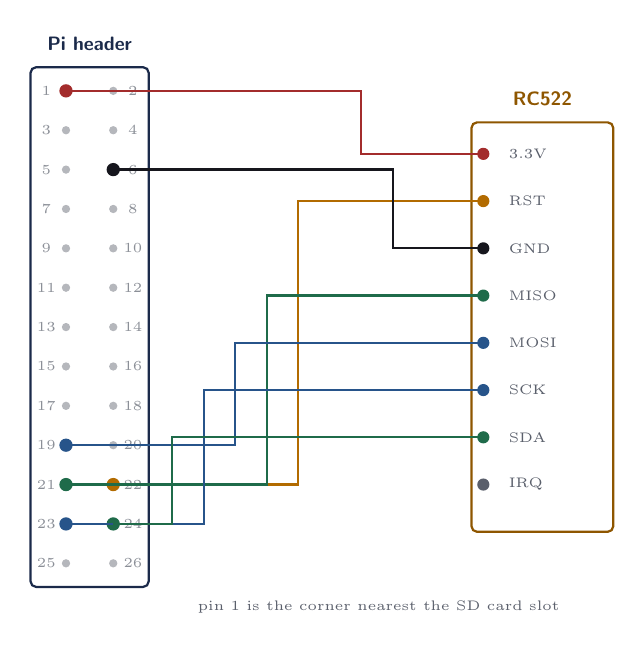
\begin{tikzpicture}[font=\scriptsize\sffamily, x=1cm, y=1cm]
  % Pi header: two columns of pins, numbered as on the board
  \draw[brewernavy, line width=0.8pt, rounded corners=2pt] (0,-0.3) rectangle (1.5,6.3);
  \node[color=brewernavy, font=\scriptsize\sffamily\bfseries] at (0.75,6.6) {Pi header};
  \foreach \y/\l/\r in {6/1/2, 5.5/3/4, 5/5/6, 4.5/7/8, 4/9/10,
                        3.5/11/12, 3/13/14, 2.5/15/16, 2/17/18,
                        1.5/19/20, 1/21/22, 0.5/23/24, 0/25/26}{
     \fill[brewergrey!45] (0.45,\y) circle (1.5pt);
     \fill[brewergrey!45] (1.05,\y) circle (1.5pt);
     \node[color=brewergrey!70, font=\tiny] at (0.2,\y) {\l};
     \node[color=brewergrey!70, font=\tiny] at (1.3,\y) {\r};
  }
  % highlight the pins we use
  \foreach \y/\x/\c in {6/0.45/brewerred, 5/1.05/brewerink, 1.5/0.45/brewerblue,
                        1/1.05/breweramber, 1/0.45/brewergreen,
                        0.5/0.45/brewerblue, 0.5/1.05/brewergreen}{
     \fill[\c] (\x,\y) circle (2.4pt);
  }
  % RC522
  \draw[breweramber!80!black, line width=0.8pt, rounded corners=2pt] (5.6,0.4) rectangle (7.4,5.6);
  \node[color=breweramber!80!black, font=\scriptsize\sffamily\bfseries] at (6.5,5.9) {RC522};
  \foreach \y/\lbl/\c in {5.2/3.3V/brewerred, 4.6/RST/breweramber,
                          4.0/GND/brewerink, 3.4/MISO/brewergreen,
                          2.8/MOSI/brewerblue, 2.2/SCK/brewerblue,
                          1.6/SDA/brewergreen, 1.0/IRQ/brewergrey}{
     \fill[\c] (5.75,\y) circle (2.2pt);
     \node[color=brewergrey, anchor=west, font=\tiny] at (5.95,\y) {\lbl};
  }
  % wires (schematic, not geometric)
  \draw[brewerred,   line width=0.8pt] (0.45,6)   -- (4.2,6)   -- (4.2,5.2) -- (5.75,5.2);
  \draw[breweramber, line width=0.8pt] (1.05,1)   -- (3.4,1)   -- (3.4,4.6) -- (5.75,4.6);
  \draw[brewerink,   line width=0.8pt] (1.05,5)   -- (4.6,5)   -- (4.6,4.0) -- (5.75,4.0);
  \draw[brewergreen, line width=0.8pt] (0.45,1)   -- (3.0,1)   -- (3.0,3.4) -- (5.75,3.4);
  \draw[brewerblue,  line width=0.8pt] (0.45,1.5) -- (2.6,1.5) -- (2.6,2.8) -- (5.75,2.8);
  \draw[brewerblue,  line width=0.8pt] (0.45,0.5) -- (2.2,0.5) -- (2.2,2.2) -- (5.75,2.2);
  \draw[brewergreen, line width=0.8pt] (1.05,0.5) -- (1.8,0.5) -- (1.8,1.6) -- (5.75,1.6);
  \node[color=brewergrey, font=\tiny, anchor=west] at (2.0,-0.55)
       {pin 1 is the corner nearest the SD card slot};
\end{tikzpicture}
\end{center}

\begin{trap}{3.3\,V, not 5\,V}
Pin 1 is 3.3\,V. Pin 2 --- \emph{directly beside it} --- is 5\,V, and it will
destroy the RC522.

Count carefully. Pin 1 is the corner nearest the SD card slot; odd numbers run
down one side, even down the other. Getting this wrong is silent, immediate and
permanent.
\end{trap}

\begin{trap}{\reg{SDA} is not I\textsuperscript{2}C here}
The RC522 board labels its chip-select pin \reg{SDA}, which is an
I\textsuperscript{2}C name. The module supports several buses and the silkscreen
reflects a different one.

For SPI, \reg{SDA} goes to \textbf{CE0, Pi pin 24}. This is the single most
common mis-wiring, and its symptom is \code{VersionReg = 0x00}.
\end{trap}

\section{Check it twice}

Before powering on, verify each wire by touching both ends, one at a time. Seven
wires, seven checks. Two minutes now saves an hour later --- and unlike code,
you cannot \code{printf} a wire.

Then power up and wait a minute.

\section{Probe it}

\begin{shell}
# on your laptop
make deploy-full
make probe
\end{shell}

\begin{verifybox}
\begin{trace}
=== RC522 wiring probe ===
Opening SPI bus 0, chip-select 0, 1 MHz, mode 0...
VersionReg   (0x37) = 0x92
TxControlReg (0x14) = 0x80

  -> WIRING OK. The RC522 is alive and talking.
     You are ready for Chapter 1 of the main book.
\end{trace}
\end{verifybox}

\hex{0x92} is the MFRC522 v2.0 identifier (\hex{0x91} is v1.0 --- also fine).
The chip is powered, on the right pins, and speaking SPI at the right clock and
mode.

\section{If it does not say that}

The probe diagnoses itself. Its three failure messages, and what they mean:

\begin{center}\small
\begin{tabular}{@{}L{0.16\linewidth}L{0.32\linewidth}L{0.44\linewidth}@{}}
\toprule
\thead{Reading} & \thead{Meaning} & \thead{Check, in order} \\
\midrule
\hex{0x00} & MISO stuck low --- the chip is not driving the line &
  Power (3.3\,V and GND); then \reg{SDA} $\rightarrow$ pin 24; then \reg{MISO}
  $\rightarrow$ pin 21 \\
\hex{0xFF} & MISO floating --- nothing connected &
  \reg{MISO} $\rightarrow$ pin 21. If connected, suspect a dead module \\
varies & noise & \textbf{Shorter wires.} Run the probe three times: if the value
  \emph{changes}, it is definitely wiring \\
\bottomrule
\end{tabular}
\end{center}

And if it fails to open SPI at all:

\begin{center}\small
\begin{tabular}{@{}L{0.40\linewidth}L{0.52\linewidth}@{}}
\toprule
\thead{Error} & \thead{Fix} \\
\midrule
\code{No such file or directory} & SPI not enabled. \code{sudo raspi-config},
  Interface Options, then \textbf{reboot} \\
\code{Permission denied} & Not in the \code{spi} group --- and remember the
  change needs a fresh login \\
\code{No gpio chip found} & You ran it on your laptop, not the Pi \\
\bottomrule
\end{tabular}
\end{center}

\begin{concept}{Why this probe exists at all}
It answers one question and nothing else: \emph{is the hardware wired correctly?}

From Volume One, Chapter 1 onwards you will be writing your own driver, and its
bugs will look exactly like wiring faults. Having a known-good, disposable
diagnostic means you never have to wonder which one you are looking at.

Keep it. Run it whenever anything hardware-shaped goes wrong. It is deliberately
ugly --- one flat method, no abstractions --- because a diagnostic you have to
debug is worthless.
\end{concept}

\section{You are done}

\begin{checkpoint}{Volume Zero complete}
\begin{shell}
ssh brewer 'hostname'          # one word, no password
cd ~/midnight-brewer && mvn test    # Tests run: 3
make deploy && make run        # runs on the Pi, aarch64
make probe                     # WIRING OK
git log --oneline              # at least one commit
git push                       # backed up
\end{shell}

Six commands, six green results. You have:

\begin{itemize}
  \item a headless Pi reachable by name, with key-only SSH;
  \item Java 21 and Maven on both machines;
  \item a project that builds and tests in seconds;
  \item a five-second deploy loop to real hardware;
  \item your work in git and on GitHub;
  \item an NFC reader answering.
\end{itemize}

None of that was specific to NFC. It is the setup for any embedded Linux project
you will ever do.
\end{checkpoint}

\vspace{1em}

Now open \textbf{Volume One} --- \emph{Building a Contactless Payment Terminal
From Scratch} --- and turn to Chapter 1. You will write an interface, build a
fake SPI bus, and test a driver with the reader unplugged.

\begin{flushright}\itshape
The environment is no longer something that can be wrong.
\end{flushright}


% ============================================================
\appendix
\part{Appendices}
\chapter{Cheat sheet}
\label{app:cheat}

One page per topic. Photocopy, print, or keep the PDF open on a second screen.

\section{The daily loop}

\begin{shell}
mvn test                      # fast, local, no hardware
make deploy && make run       # onto the real Pi
make probe                    # is the reader still alive?
git add -A && git commit -m "feat: ..." && git push
\end{shell}

\section{SSH}

\begin{shell}
ssh brewer                          # log in (alias from ~/.ssh/config)
ssh brewer 'uptime'                 # run one command, come straight back
ssh -v brewer                       # verbose -- diagnose auth failures
exit                                # or Ctrl-D

scp file.txt brewer:~               # copy a file over
scp -r brewer:~/logs ./logs         # copy a folder back
rsync -a --delete src/ brewer:dst/  # mirror a folder (note trailing slashes)
\end{shell}

\subsection*{\texttt{\textasciitilde/.ssh/config}}

\begin{trace}
Host brewer
    HostName brewer.local
    User martin
    IdentityFile ~/.ssh/id_ed25519
    ServerAliveInterval 30
    ServerAliveCountMax 6
\end{trace}

\subsection*{Key setup, from scratch}

\begin{shell}
ssh-keygen -t ed25519 -C "martin@laptop"    # once, ever
ssh-copy-id martin@brewer.local             # once per machine
chmod 700 ~/.ssh && chmod 600 ~/.ssh/*      # if keys are ignored
\end{shell}

\section{Git}

\begin{shell}
git status                    # what changed?
git diff                      # show the actual changes
git diff --staged             # ... that are staged
git add -A                    # stage everything
git add -p                    # stage interactively, hunk by hunk
git commit -m "feat: ..."     # save point
git push                      # back it up
git log --oneline -10         # last ten commits
git log --oneline -- path/to/File.java     # history of one file
git show HEAD                 # what was in the last commit
git checkout -- file.java     # DISCARD my changes to this file
git reset --soft HEAD~1       # undo the last commit, keep the changes
git stash / git stash pop     # shelve work temporarily
\end{shell}

\subsection*{Message prefixes}

\begin{trace}
feat:   a new capability
fix:    a bug fixed
chore:  housekeeping, build, dependencies
docs:   documentation
test:   tests only
\end{trace}

\section{Maven}

\begin{shell}
mvn test                      # compile + run tests
mvn -q compile                # compile quietly
mvn clean                     # delete target/
mvn clean test                # when you suspect stale output
mvn test -Dtest=FooTest       # one test class
mvn dependency:copy-dependencies -DincludeScope=runtime
mvn dependency:tree           # why is THAT jar on my classpath?
\end{shell}

\subsection*{Running things}

\begin{shell}
java -cp target/classes com.midnightbrewer.ToolchainCheck
java -cp "target/classes:target/dependency/*" com.midnightbrewer.diag.SpiProbe
\end{shell}

\section{The Pi}

\begin{shell}
# identity and health
hostname
cat /proc/device-tree/model; echo
free -h                       # memory
df -h /                       # disk
vcgencmd measure_temp         # temperature
uptime                        # load and how long it has been up

# hardware
ls -l /dev/spidev0.0          # SPI device present?
groups                        # am I in spi and gpio?
lsmod | grep spi              # SPI kernel modules loaded

# services and logs
sudo systemctl status ssh
journalctl -u ssh -n 50       # last 50 lines of a service's log
journalctl -f                 # follow everything, live
dmesg | tail -20              # kernel messages (undervoltage shows here)

# packages
sudo apt update && sudo apt full-upgrade -y
sudo apt install -y <package>

sudo reboot
sudo shutdown -h now          # ALWAYS before touching wiring
\end{shell}

\section{Terminal}

\begin{shell}
pwd                     # where am I?
ls -la                  # what is here, including hidden
cd -                    # back to the previous directory
find . -name "*.java"   # find files by name
grep -rn "TODO" src/    # search a tree, with line numbers
chmod +x script.sh      # make executable
du -sh *                # what is taking up space
history | grep ssh      # what was that command last week?
\end{shell}

\begin{center}\small
\begin{tabular}{@{}ll@{}}
\toprule
\textbf{Tab} & complete a name (and prove it exists) \\
\textbf{Up} & previous command \\
\textbf{Ctrl-R} & search history \\
\textbf{Ctrl-C} & stop the running program \\
\textbf{Ctrl-D} & end input / log out \\
\textbf{Ctrl-A / Ctrl-E} & start / end of line \\
\bottomrule
\end{tabular}
\end{center}

\section{Pin reference}

\begin{center}\small
\begin{tabular}{@{}llll@{}}
\toprule
\thead{RC522} & \thead{Pi pin} & \thead{BCM} & \thead{Function} \\
\midrule
\reg{3.3V} & 1  & --- & power (\textbf{never pin 2}) \\
\reg{GND}  & 6  & --- & ground \\
\reg{MOSI} & 19 & 10  & Pi $\rightarrow$ chip \\
\reg{MISO} & 21 & 9   & chip $\rightarrow$ Pi \\
\reg{RST}  & 22 & 25  & reset \\
\reg{SCK}  & 23 & 11  & clock \\
\reg{SDA}  & 24 & 8   & chip select (CE0) \\
\reg{IRQ}  & --- & --- & not connected \\
\bottomrule
\end{tabular}
\end{center}

\section{Values worth memorising}

\begin{center}\small
\begin{tabular}{@{}ll@{}}
\toprule
\hex{0x91} / \hex{0x92} & healthy RC522 version byte \\
\hex{0x00} & MISO stuck low --- power or wiring \\
\hex{0xFF} & MISO floating --- not connected \\
\code{aarch64} & correct Pi architecture (64-bit) \\
\code{Tests run: 3} & the starter pack's test count \\
\bottomrule
\end{tabular}
\end{center}

\chapter{When it does not work}
\label{app:trouble0}

Indexed by \textbf{what you see on screen}. Search for your error message here
before searching the internet --- almost every setup failure has a known cause
and a one-line fix.

\section{First, three questions}

Before diagnosing anything, answer these. They resolve most problems on their
own.

\begin{enumerate}
  \item \textbf{Which machine am I on?} Run \code{hostname}. Half of all setup
        confusion is the right command on the wrong machine.
  \item \textbf{Where am I?} Run \code{pwd}. The other half is the right command
        in the wrong directory.
  \item \textbf{Did I reboot / log out?} SPI needs a reboot. Group membership
        needs a fresh login. Both fail silently until you do.
\end{enumerate}

\section{Cannot reach the Pi}

\begin{traptable}
\code{ssh: Could not resolve hostname brewer.local} &
  mDNS not working. Find the IP from your router and use it directly; then put
  the IP in \code{HostName} in \code{\textasciitilde/.ssh/config}. \\
\code{ssh: connect to host ... port 22: Connection refused} &
  The Pi is up but SSH is not running --- you did not enable it in Imager.
  Re-flash. \\
\code{... Operation timed out} &
  The Pi is not on the network at all. Wi-Fi credentials, 5\,GHz, wireless
  country, or power. \\
\code{ping} works, \code{ssh} does not &
  SSH not enabled. Re-flash with the Services tab ticked. \\
Never appeared at all &
  Re-flash rather than diagnose. Five minutes, and it fixes most cases. \\
Worked yesterday, not today &
  DHCP gave it a new address. Use the hostname, or set a static lease in your
  router. \\
\end{traptable}

\subsection*{\texttt{REMOTE HOST IDENTIFICATION HAS CHANGED}}

\begin{trace}
@@@@@@@@@@@@@@@@@@@@@@@@@@@@@@@@@@@@@@@@@@@@@@@@@@@@@@@@@@@
@    WARNING: REMOTE HOST IDENTIFICATION HAS CHANGED!      @
@@@@@@@@@@@@@@@@@@@@@@@@@@@@@@@@@@@@@@@@@@@@@@@@@@@@@@@@@@@
\end{trace}

You reflashed the Pi (new host key), or your router gave that address to a
different device. Remove the stale entry:

\begin{shell}
ssh-keygen -R brewer.local
ssh-keygen -R 192.168.1.42      # also the IP, if you used it
\end{shell}

\begin{trap}{Never disable host checking to make this go away}
\code{StrictHostKeyChecking=no} silences the warning permanently and removes the
only protection you have against connecting to an impostor.

Remove the \emph{specific} stale entry instead. It is one command.
\end{trap}

\section{SSH keys still ask for a password}

\begin{traptable}
Asks for a password after \code{ssh-copy-id} &
  Permissions. On the Pi: \code{chmod 700 \textasciitilde/.ssh} and
  \code{chmod 600 \textasciitilde/.ssh/authorized\_keys}. SSH ignores loose
  permissions \emph{silently}. \\
Works for \code{ssh}, not for \code{scp}/\code{rsync} &
  Those read \code{\textasciitilde/.ssh/config} too --- check the \code{Host}
  alias matches what you are typing. \\
\code{Permission denied (publickey)} after disabling passwords &
  The key was never installed correctly. If you can no longer get in, mount the
  SD card on your laptop and re-enable \code{PasswordAuthentication}, or
  re-flash. \\
Prompts for the key passphrase every time &
  Add it to the agent: \code{ssh-add \textasciitilde/.ssh/id\_ed25519}
  (macOS: \code{ssh-add --apple-use-keychain}). \\
\end{traptable}

Diagnose with \code{ssh -v brewer} --- it prints which keys were offered and what
the server did with them.

\section{Java and Maven}

\begin{traptable}
\code{java: command not found} &
  Not installed, or not on your \code{PATH}. Reopen your terminal after
  installing. \\
\code{mvn -v} reports a different Java than \code{java -version} &
  Maven uses \code{JAVA\_HOME}. Set it: \code{export JAVA\_HOME=\$(/usr/libexec/java\_home -v 21)} on macOS, or
  \code{export JAVA\_HOME=/usr/lib/jvm/java-21-openjdk-arm64} on the Pi. \\
\code{class file has wrong version 65.0} &
  Compiled with a newer Java than you are running. Check both machines are 21. \\
\code{Tests run: 0} &
  Tests not found. Class must end in \code{Test} and live under
  \code{src/test/java}. \\
\code{Non-parseable POM} &
  XML error. A comment containing \code{--} is the usual culprit; it is illegal
  inside \code{<!-- -->}. \\
Build downloads forever &
  First build only. If it repeats, delete \code{\textasciitilde/.m2/repository}
  and try once more. \\
\code{ClassNotFoundException} at runtime &
  Classpath missing the dependency jars. Use
  \code{-cp "target/classes:target/dependency/*"} and run
  \code{make deploy-full}. \\
\end{traptable}

\section{SPI and the reader}

\begin{traptable}
\code{/dev/spidev0.0: No such file} &
  SPI not enabled, or you did not reboot after enabling it. \\
\code{Permission denied} on spidev &
  Not in the \code{spi} group --- \emph{or} you are, but have not logged out and
  back in since. \\
\code{No gpio chip found} &
  You are running on your laptop, not the Pi. \\
\code{VersionReg = 0x00} &
  MISO stuck low. Power (3.3\,V, not 5\,V), then \reg{SDA} $\rightarrow$ pin 24,
  then \reg{MISO} $\rightarrow$ pin 21. \\
\code{VersionReg = 0xFF} &
  MISO floating. Not connected, or dead module. \\
Version changes between runs &
  Wire length. \textbf{Shorten the jumpers.} This is not a code problem. \\
Device or resource busy &
  A previous run is still holding SPI. \code{ssh brewer 'pkill java'}. Use
  \code{run.sh} (which passes \code{ssh -t}) so Ctrl-C actually reaches it. \\
\end{traptable}

\section{The Pi misbehaves}

\begin{traptable}
Random reboots, or a rainbow square &
  Undervoltage. Replace the power supply \emph{and} the cable. Confirm with
  \code{dmesg | grep -i voltage}. \\
SSH dies during a build &
  Out of memory --- the kernel killed \code{sshd}. Add swap
  (Chapter~\ref{ch:pisetup}) and build on your laptop. \\
Everything is extremely slow &
  A slow or failing SD card. Check with \code{dmesg | grep -i mmc}. \\
\code{No space left on device} &
  \code{df -h /}. Clear caches with \code{sudo apt clean} and delete old
  \code{target/} folders. \\
Filesystem is read-only &
  The card is failing or was corrupted by a power cut. Back up and re-flash. \\
\end{traptable}

\section{Git and GitHub}

\begin{traptable}
\code{Permission denied (publickey)} on push &
  Your public key is not on GitHub. Test with \code{ssh -T git@github.com}. \\
\code{Support for password authentication was removed} &
  You are using an HTTPS remote. Switch to SSH:
  \code{git remote set-url origin git@github.com:USER/REPO.git}. \\
\code{failed to push some refs} &
  The remote has commits you do not. \code{git pull --rebase} then push. \\
\code{Please tell me who you are} &
  Set \code{user.name} and \code{user.email} --- see
  Chapter~\ref{ch:laptop}. \\
Stuck in a full-screen editor &
  That is vim. Press Escape, type \code{:q!}, press Enter. Then
  \code{git config --global core.editor nano}. \\
Committed a secret &
  Assume it is compromised. Rotate the key or password. Deleting it in a later
  commit does not remove it from history. \\
\end{traptable}

\section{The deploy loop}

\begin{traptable}
Changes have no effect &
  Stale classes. \code{mvn clean compile \&\& make deploy-full}. \\
\code{rsync: command not found} &
  Install it on \emph{both} machines. \\
Files land in \code{classes/classes/} &
  Missing trailing slash on the rsync source. \code{target/classes/} means
  ``the contents of''. \\
Ctrl-C does not stop the remote program &
  Use \code{ssh -t}. \code{run.sh} already does. \\
\code{make: command not found} &
  macOS: install the Xcode command line tools. Linux:
  \code{sudo apt install make}. \\
\end{traptable}

\section{Still stuck?}

Narrow it down before asking anyone, including a search engine:

\begin{enumerate}
  \item \textbf{Does it work on the other machine?} If \code{mvn test} passes on
        your laptop but fails on the Pi, the problem is environmental, not code.
  \item \textbf{Did it ever work?} If yes, \code{git diff} shows exactly what
        changed since.
  \item \textbf{What is the smallest thing that fails?} \code{ssh brewer
        'echo hi'} before \code{make deploy}. Test one layer at a time.
  \item \textbf{Read the whole error.} The useful line is often the third, not
        the first --- and in Java the useful part is usually \code{Caused by:}
        near the bottom.
\end{enumerate}

\begin{concept}{Bisect, do not stare}
The habit that separates fast debugging from slow: instead of reading code
hoping to spot the fault, \textbf{find the boundary between what works and what
does not}.

\code{ssh} works but \code{scp} does not $\rightarrow$ it is the config, not the
network. \code{mvn test} passes but \code{make run} fails $\rightarrow$ it is the
classpath, not the code.

Each check halves the search space. Four checks turn sixteen possibilities into
one.
\end{concept}


% ============================================================
\backmatter
\cleardoublepage
\phantomsection
\addcontentsline{toc}{chapter}{Index}
\printindex

\end{document}
